\documentclass[11pt,reqno]{article}
%\documentclass{amsart}
\usepackage{amsmath,amssymb,amsfonts,amsthm,bbm,mathrsfs,verbatim} % Typical maths resource packages
\usepackage[misc]{ifsym}
\usepackage{bbm}
\usepackage{graphics}                 % Packages to allow inclusion of graphics
\usepackage{graphicx}
\usepackage{float}
\usepackage{array}
\usepackage{mathtools}
\usepackage{blkarray}
%\floatstyle{boxed}
%\restylefloat{figure}
\usepackage{color}                    % For creating coloured text and background
\usepackage{hyperref}                 % For creating hyperlinks in cross references
\usepackage{makeidx}
\usepackage{caption}
\usepackage{bbm}
\usepackage{algorithmic}
%\usepackage{natbib}
\usepackage{authblk}
%\graphicspath{ {./Desktop/} }
\usepackage{amsmath} % for \boxed and \smash[b] macros
\usepackage{booktabs}% for \midrule and \cmidrule macros
\newcommand\headercell[1]{%
	\smash[b]{\begin{tabular}[t]{@{}c@{}} #1 \end{tabular}}}

\newtheorem*{acknowledgement}{Acknowledgement}

\newtheorem{theorem}{Theorem}[section]
\newtheorem{proposition}[theorem]{Proposition}
\newtheorem{corollary}[theorem]{Corollary}
\newtheorem{lemma}[theorem]{Lemma}
\theoremstyle{definition}
\newtheorem{remark}[theorem]{Remark}
\newtheorem{definition}[theorem]{Definition}
\newtheorem{example}[theorem]{Example}
\newtheorem{assumption}[theorem]{Assumption}
\newtheorem{notation}[theorem]{Notation}
\newtheorem{algorithm}[theorem]{Algorithm}
\newcommand{\rank}{\text{rank}}



\def\R{{\mathbb R}}
\def\X{{\mathbb X}}
\newcommand\red[1]{\textcolor{red}{#1}}
\newcommand\blue[1]{\textcolor{blue}{#1}}
\def\U{{\cal U}}
\def\Ut{\bar{\U}}
\def\Q{{\cal Q}}
\def\J{{\cal J}}
\def\Jb{\bar{\J}}
\def\Jo{\J^{(1)}_{\delta}}
\def\Jt{\J^{(2)}_{\delta}}
\def\wc{\rightharpoonup}
\def\WI{W_{0}^{1,2}(I)}
\def\WIG{W^{1,2}(I)}

\def\HA{{\mathbb H}_{K_{a}}}
\def\HD{{\mathbb H}_{K_{d}}}
\def\la{\langle}
\def\ra{\rangle}
\newcommand\A[2]{A_{#1}(#2)}

\newcommand{\ud}{\, {\rm d}}
\newcommand{\nnb}{\nonumber}

\newcommand\M[1]{M^{(#1)}}
\newcommand\MH[1]{\hat{M}^{(#1)}}
\newcommand\f[1]{f^{(#1)}}
\newcommand\fH[1]{\hat{f}^{(#1)}}
\newcommand\p[1]{p^{(#1)}}
\newcommand\pH[1]{\hat{p}^{(#1)}}

\newcommand\grad[1]{\nabla \, #1}
\newcommand\dv[1]{\nabla \cdot #1}
\newcommand\curl[1]{\nabla \times #1}
\newcommand\cc[1]{\nabla \times\nabla \times #1}
\newcommand\dt[1]{\frac{\partial}{\partial t} #1}
\newcommand\dtdt[1]{\frac{\partial^2}{\partial t^2} #1}

\def\e{\varepsilon}

\setlength{\affilsep}{2em}




\textheight 215mm \textwidth 170mm
\oddsidemargin -1pt \evensidemargin -1pt
\marginparwidth 10pt \topmargin -22pt

\begin{document}
\title{Partial integro-differential equations for default probabilities of L\'evy-driven Ornstein-Uhlenbeck asset processes and applications to credit risk}
	
\author{K. Georgiou, A.N. Yannacopoulos}
\maketitle
\tableofcontents



\begin{abstract}
In this paper we consider applications of stochastic processes and their hitting times to Probability of Default (PD) estimations. In particular, we develop a framework based on Partial Integro-differential equations, that can be used for estimating PD processes with variable initial time and maturities, both of which are of imperative to credit risk modelling under the International Financial Reporting Standards (IFRS) 9. Finally, we use appropriate numerical methods for examples specific to provisioning under IFRS 9, as well as other credit risk modelling problems.
\end{abstract}

\section{Introduction}
One of the main issues currently concerning financial institutions is the implementation of the new International Financial Reporting Standards (IFRS) 9. Due to the financial crisis, the purpose of the updated standards is to introduce a framework under which institutions forecast credit losses (for loan provisioning purposes). Specifically, “under the impairment approach in IFRS 9 it is no longer necessary for a credit event to have occurred before credit losses are recognised. Instead, an entity always accounts for expected credit losses, and changes in those expected credit losses. The amount of expected credit losses is updated at each reporting date to reflect changes in credit risk since initial recognition and, consequently, more timely information is provided about expected credit losses”. Furthermore, "the objective of the impairment requirements is to recognise lifetime expected credit losses for all financial instruments for which there have been significant increases in credit risk since initial recognition — whether assessed on an individual or collective basis — considering all reasonable and supportable information" (IFRS 9 Red Book). Further details and research are given in \cite{beerbaum2015significant} and \cite{xu2016estimating}. Hence, loan provisioning regulations under IFRS 9, require financial institutions to consider expected losses based on the current credit state of each loan and the possible future losses. This estimation requires knowledge of the lifetime Probability of Default (PD) for all loan exposures, as well as additional risk parameters such as the Loss Given Default (LGD) and the Exposure at Default (EAD). The estimation of future losses (i.e. forward looking provisions) can therefore be tackled by employing the theory of stochastic processes and their dynamics.
\par Under IFRS 9, it is now mandatory for financial institutions to classify loans into three distinct categories, known as the IFRS 9 Stages. Specifically, Stage 1 loans are considered performing, Stage 2 contains loans which have displayed a significant increase in credit risk and Stage 3 contains all Non-Performing loans (NPLs), considered to have defaulted. As mentioned, the insitutions must forecast future losses specifically for the Stage 2 loans, which are considered to be at risk. In the present work, we will focus on portfolios of corporate and small business loans, where it is common practice to consider the company's assets to be governed by a stochastic process. Under this assumption, the PD associated with each loan depends on the underlying asset process and we can define the PD as the probability that the asset process falls below a fixed threshold. 
\par More specifically, we will consider an Ornstein - Uhlenbeck (OU) process with a jump for the modelling of the asset process. The OU process has been used extensively in seminal work related to ruin probabilities and is considered an industry standard. Important theoretical background of such processes and their properties are given in \cite{applebaum2009levy} and \cite{oksendal2007applied}. The jump process will account for abrupt changes in the assets, which are very common in practice and are closely related to loan defaults. Obtaining the term structure of the PD process, based on the stochastic asset model, will allow us to then estimate lifetime provisions.
\par An important aspect of the present work is the initial technical analysis of the underlying stochastic jump process, i.e. continuity and weak differentiability. These preliminary results allow us to consider two separate cases for the PD of the asset process:
\begin{itemize}
	\item A variable starting time and constant time horizon.
	\item A variable time horizon and constant starting time.
\end{itemize}
Our results present generalizations of the ruin probabilities analyzed in \cite{mishura2016ruin} and \cite{moller1995stochastic}, and we prove that, under certain conditions, equivalent partial integro-differential equations can be obtained for the dynamics of the PD process.
\par The above methodology will be used to consider real-life examples of loan provisioning calculations, creating a full PD and provisions framework under IFRS 9. Finally, we note that, even though motivated by credit risk modelling, the arguments presented are applicable to more general problems related to similar probabilities of underlying stochastic processes. 



\section{Preliminaries}
In this section we introduce and define the required framework and results that will be used throughout the remainder of this work. In particular, we focus continuous and discrete stochastic processes and important results. 
\subsection{L\'evy processes}
Throughout this paper, we have abopted the notation used in \cite{oksendal2007applied}. We start by defining a L\'evy process:

\begin{definition}[L\'evy process]
	A L\'evy process $\{L_t\}_{t \geq 0} $ is a stochastic process for which the following conditions hold:
	\begin{itemize}
		\item $L_0=0$.
		\item $L$ has independent and stationary increments, i.e. if $ t >s$ then $L_t-L_s$ is independent from $ L_s$ and $L_t-L_s \stackrel{D}{=} L_{t-s}$.
		\item  $L$ is stochastically continuous, i.e for all $\epsilon >0 $ and all $ s >0$ we have $$\lim_{t \rightarrow s} \mathbb{P}(|X(t)-X(s)|>\epsilon)=0.$$
	\end{itemize}
\end{definition}

A consequence of the above definition is the celebrated It\^o - L\'evy decomposition. First, we define the following required quantities:

\begin{definition}
	Let $L_t$ be a L\'evy process, whose jump is defined as $\Delta L_t = L_t - L_{t_-}$. Furthermore, let $\textbf{B}_0$ be the family of Borel sets $U \subset \mathbb{R} $, whose closure does not contain 0. Then, for $U \in \textbf{B}_0$, define the Poisson random measure of the L\'evy process $L_t$ by: 
	$$ N(t,U) = \sum_{0 < s \leq t } \chi (\Delta L_s).$$ 
\end{definition}
The Poisson random measure represents the number of jumps of size $\Delta L_s \in U$, which occur up to time $t$. We can therefore define the intensity of the jumps as follows:
\begin{definition}
	The intensity of a L\'evy jump process $L_t$, known as the L\'evy measure of $L_t$ is defined as:
	$$\nu(U) = \mathbb{E}[N(1,U)],$$
	where, as above, $U \in \textbf{B}_0$.
\end{definition}
A useful consequence of the above definitions is that if $\nu$ is the L\'evy measure of a simple Compount Poisson Process with intensity $\lambda$ and jump size density $f(z)$, then we have that $$ \nu(U) = \lambda f(U).$$ To this end, we will employ the following result in the subsequent sections, due to \cite{kyprianou2006introductory}:

\begin{theorem}
	Consider the Poisson random measure  $N(t,U)$, with $U \in \textbf{B}_0$, and corresponding L\'evy measure $\nu(U)$. Then the process:
	$$ X_t = \int_{[0,t]} \int_{B} z N(ds,dz), $$
	where $B \in \mathcal{B}(\mathbb{R})$ is a Compound Poisson Process with intensity $\nu(B)$ and jump distribution $\frac{\nu(dx)|_B}{\nu(B)^{-1}}$.
\end{theorem}
We can now present the following theorem:
\begin{theorem}[It\^o - L\'evy decomposition]
	Let $\{L_t\}_{t \geq 0}$ be a L\'evy process. Then, we have 
	\begin{eqnarray}
		L_t = bt + \sigma B_t + \int_{|z|<1} z \tilde{N}(t,dz) + \int_{|z| \geq1} z N(t,dz), 
	\end{eqnarray}
	for $ t \geq 0 $, where $b, \sigma \in \mathbb{R}$, $B_t$ is a Brownian motion and $\tilde{N}(t,dz):=N(t,dz)- \nu(dz)t$ is the compensated Poisson measure. 	
\end{theorem}
More generally, we can define the stochastic process $ X(t)$, as: 
\begin{eqnarray}
	dX_t=a(t)dt + \sigma(t)dB(t) + \int_{|z|<1} H(t,z) \tilde{N}(dt,dz) + \int_{|z| \geq1} H(t,z) N(dt,dz),
\end{eqnarray}
known as L\'evy - It\^o processes. Moreover, by combining the compensator with the drift term the above can be written as: 
\begin{eqnarray}
	dX_t=a(t)dt + \sigma(t)dB(t) + \int_{z \in \mathbb{R}} H(t,z) N(dt,dz).
\end{eqnarray}
We will adopt this formulation throughout the remainder of this work.

In order to analyze the dynamics of the resulting processes, we will employ the It\^o formula for functions of such L\'evy - It\^o processes. However, in many cases, differentiability conditions required for the standard It\^o formula may not hold. We therefore must consider versions of the formula applicable to functions for which we can only prove differentiability in the weak sense. These results are provided in the Appendix. Such solutions are often referred to as viscocity solutions; more details are provided in subsequent sections. We will show in the following sections that the PD process satisfies a partial integro-differential equation in the weak sense, allowing us to find numerical solutions, which is the main interest for applications considered in this work. 

\subsection{The Ornstein-Uhlenbeck process}

In its simplest form the Ornstein-Uhlenbeck (OU) process $G_t$ is defined as the stochastic process satisfying: 
\begin{eqnarray}\label{ou}
	dG_t=k(\theta - G_t)dt + \sigma dB_t, \,\, G_s=x, 
\end{eqnarray}
for some known $x$, where, as above, $B_t$ represents the standard Brownian motion and $k, \theta$ and $\sigma$ are positive real constants. The OU process is a mean-reverting, Gaussian and Markov process, which is also temporally homogeneous. We can therefore equivalently write (\ref{ou}) as:
\begin{eqnarray}
	dG_u=k(\theta - G_t)du+ \sigma dB_u, \,\, G_0=x,
\end{eqnarray}
where $u = t-s$. 
We note that the process satisfying (\ref{ou}) when $\theta \neq 0$ is often also referred to as the Vasicek model \cite{vasicek1977equilibrium}. Employing It\^o's formula we can obtain the solution to the above SDE:
$$ G_t = x e ^{-kt}+ \theta(1-e^{-kt}) + \sigma \int_{0}^{t} e^ {-k(t-u)}dB_u,$$
from which is it easy to see that $G_t \sim N(\theta + (x - \theta) e^{-kt}, \sigma^2(1-e^{-2kt})/2k).$
These properties are what make this particular family of processes widely used in many applications. We will also need the following regarding the transition density and hitting time for the OU process.

\begin{theorem}\label{td}
	The transition density of the OU process, with initial condition $G_0=x$ is given by: 
	\begin{eqnarray}
		p(t,x,y) = \sqrt{\frac{k}{\pi \sigma^2 (1-e^{-2kt})}} \exp\Big(-\frac{k(y-x e^{-kt})^2}{\sigma^2 (1-e^{-2kt})}\Big).
	\end{eqnarray}
\end{theorem}

\begin{theorem}\label{sp} For the OU process as defined in (\ref{ou}), the density of the hitting time $u := \inf\{t>0: G_t^x \leq 0\}$ can be defined via the Volterra equations. We refer the reader to \cite{lipton2018first}.
\end{theorem}


\subsection{Markov chains}
In this paper, we will also consider regime switching models and their applications in provision calculations. To this end, we introduce the following important definitions related to Markov chains.

\begin{definition}[Markov chain]
	A discrete state Markov chain $M,$ defined on a state space $S$, of cardinality $|S|=n < \infty$, is a stochastic process $\{X_t: t \in \mathbb{N}\}$, such that 
	\begin{equation}
		\mathbb{P} (X_{t} = s_t | X_{t-1} = s_{t-1}, \cdots, X_{1}=s_1) = \mathbb{P} ( X_{t}=s_t  | X_{t-1}=s_{t-1}) 
	\end{equation}
	for any states $s_i\in S$. 
\end{definition}
For a general Markov chain, we will use the notation $M=(S,P)$, with $S$ defined as above and $P=(P_{i,j})_{i,j=1,\dots n}$ is the row-stochastic transition matrix of the Markov Chain, whose entries $P_{i,j}$ reflect the conditional probability of transition from one state of the chain to another, i.e $P_{i,j}=\mathbb{P}(X_{t+1}=j | X_t=i)$, for a fixed $n \in {\mathbb N}$. More generally, the powers of the transition matrix, $P^k$, for $k \in \mathbb{Z}_+$ give the $k-$step transition probabilities $P^k_{i,j}=\mathbb{P}(X_{t+k}=j | X_t=i)$.
\par For the Markov chain $M=(S,P)$, we say that a state $i$ is transient if, given that the chain starts at $i$, it is possible, but not certain, that the chain will return to $i$. Equivalently, there exists a non-zero probability that the chain will never return to $i$. On the other hand, a state $i$ is defined as absorbing if $P_{i,i}=1$, i.e. the probability of transitioning from $i$ to any other state is zero. 
\par In subsequent sections, we will show that, in order to obtain the dynamics of the PD process under the regime switch model, we require the infinitesimal generator of the underlying process. To this end first define the Generator of the Markov process.

\begin{definition}
	For the discrete Markov chain $M=(S,P)$, we can define the generator matrix $Q =(Q_{ij})_{i,j=1,\dots n}$ by: 
	\begin{eqnarray}
		Q = \lim_{t \downarrow 0 } \frac{ P_t - I_{n \times n }}{t},
	\end{eqnarray}
where $I_{n \times n}$ is the $n \times n$-dimensional identity matrix.
Alternatively, we can write as in \cite{zhu2015feynman}:
\begin{eqnarray}
	\mathbb{P}(X(t+\delta)=j | X(t)=i) = \begin{cases}
		q_{ij}\delta + o(\delta), \,\ i \neq j\\
		1 + q_{ii} \delta + o(\delta),
	\end{cases}
\end{eqnarray}
as $\delta \downarrow 0$, and where $\sum_{i \in S} q_{ij}=0$, with $q_{ij} \geq 0$ for $i\neq j$. 
\end{definition}
Finally, the relationship between the transition matrix $P$ and generator $Q$ of a Markov chain is given by: 
 \begin{eqnarray}
 	P = \exp{(Q)} = I + Q + \frac{Q^2}{2!} + \dots .
 \end{eqnarray}
The above can also be generalized to the $k-$step transition matrix, i.e. $P(k) = \exp{(kQ)}$. 

\section{Stochastic models for assets and Probability of Default}
\par In this section, we present the models that will be considered for the asset process. We focus on Ornstein-Uhlenbeck processes and present a standard case and an extension under a regime switching framework. We also define the Probability of Default (PD) as a function of the initial position of the asset process, as well as both the starting and maturity time, each of which find applications in credit risk modelling. 
\subsection{Ornstein-Uhlenbeck model for asset processes}
We can generalize (\ref{ou}) by replacing the stochastic term with a L\'evy -It\^o process, therefore obtaining the form below, which will be used througout the remaining of our analysis. This is known as a L\'evy-driven Ornstein-Uhlenbeck process. 
\begin{definition} A L\'evy-driven Ornstein-Uhlenbeck process is a stochastic process satisfying the stochastic differential equation:
	\begin{eqnarray}\label{gou}
		dG_t=k(\theta - G_t)dt + \sigma dB_t +  \int_{z\in \mathbb{R}} z N(dt,dz), \,\,\,\ G_s = x
	\end{eqnarray}
	where $k, \theta, \sigma \in \mathbb{R}$.
\end{definition}
This newly-defined stochastic process has two sources of randomness; the continuous Brownian motion $B_t$ and the discontinuous L\'evy jump term. It can be shown that the jump term is a compound Poisson process with arrival rate $\lambda=\nu(\mathbb{R})$ and jump distribution $f(dz)=\lambda^{-1} \nu(dz)$. For in depth analysis of integrals with respect to Poisson measures and their properties we refer the interested reader to e.g. \cite{kyprianou2006introductory}. It is also important to note that time-homogeneity still holds and therefore we can write (\ref{gou}) as: 
\begin{eqnarray} 
	\label{gou1}
	dG_u=k(\theta - G_u)du + \sigma dB_u +  \int_{z\in \mathbb{R}} z N(du,dz), \,\,\,\ G_0 = x
\end{eqnarray}
again having used the transformation $u = t-s$. 
\par Such models have been considered in past research and applications. Work has been done in the continuous OU case and the Merton model, as well as in cases incorporating jumps (see e.g. \cite{barndorff2001non}, \cite{hull2004merton}) and particularly in applications to credit risk modelling and pricing. \cite{schoutens2010levy} gives an extensive analysis of L\'evy processes and their use for asset process modelling, credit derivatives pricing and more. In \cite{onalan2009financial} and \cite{luciano2006multivariate} the authors consider a L\'evy-driven OU process, and L\'evy multivariate models for assets processes. The former fits the model parameters to the General Motors stock price, while the latter considers many different indices, obtaining suprisingly accurate results. We also refer the interested reader to \cite{ballotta2016multivariate} for a detailed analysis of the properties of the multivariate model. Seminal work has also been done in the study of L\'evy-driven OU processes in \cite{barndorff2001non}.
Finally, well-documented numerical methods exist for the calibration of stochastic models with jumps, such as the Yuima framework for stochastic differential equations in R statistical language (\cite{brouste2014yuima}).

\begin{definition}\label{PD_def}
	For the stochastic process $G_t^x$, satisfying (\ref{gou}), we define the Probability of Default function $\Psi: \mathbb{R}_+^3 \rightarrow [0,1]$ by:
	\begin{eqnarray}
		\Psi(G_s,s,t)\equiv \Psi(x,s,t) = \mathbb{P}(\inf_{\substack{s \leq r \leq t}} G_r^x \leq 0) \equiv \mathbb{P}(\inf_{\substack{s \leq r \leq t}} G_r \leq 0 | G_s=x) 
	\end{eqnarray} and the corresponding survival probability $\Phi: \mathbb{R}_+^3 \rightarrow [0,1]$ by:
	\begin{eqnarray}
		\Phi(x,s,t) = 1- \Psi(x,s,t)=\mathbb{P}(\inf_{\substack{s \leq r \leq t}} G_r^x > 0).
	\end{eqnarray}
\end{definition}
Furthermore, using the time homogeneity property, enjoyed by all three of the aforementioned processes, we see that the PD processes can be written more succinctly as: 
\begin{eqnarray}
	\Psi(x,0,u)  = \mathbb{P}\big(\inf_{\substack{r \leq u}} G_r^x \leq 0\big) \equiv \mathbb{P}\big(\inf_{\substack{ r \leq u}} G_r \leq 0 | G_0=x\big) 
\end{eqnarray}
\begin{eqnarray}
	\Phi(x,0,u) = 1- \Psi(x,0,u)=\mathbb{P}(\inf_{\substack{ r \leq u}} G_r^x > 0).
\end{eqnarray}
Note that when fixing the starting time we will write $\Psi(x,t;s)$ and when fixing the maturity $\Psi(x,s;t)$. The dependency on the parameters may also be dropped, when there is no risk of confusion. Furthemore, in the case of the regime switching and stochastic volatilty models for the asset processes, we have to average over the possible values of the latent variables to obtain the final PD values. Alternatively, if the value of the latent variable is measurable, we can introduce a condition in the definition of the PD. More details on this process and the corresponding numerical schemes are given in the sections below. 
\par The PD model proposed is based on the standard definition of the ruin probability. In our calculations in subsequent sections, we will need the expressions for the transition density $p(t,x,y)$, as well as the hitting time $u := \inf\{t>0: G_t^x \leq 0\}$ of the standard OU process, $Q(x,u)$. These are given in the Appendix. An important remark based on these results, which we will be used in the following results, is that the transition and hitting time densities are continuous and differentiable functions of $x$ and $t$. 

\subsection{Regime switching OU asset process}
%\subsubsection{Regime switching model}
As mentioned, loan exposures under IFRS 9 are classified into three Stages. Each of these Stages correspond to a given level of risk, with the most noteworthy change due to the regulation being the introduction of Stage 2 loans, which have exhibited a significant increase in credit risk (which can be defined by the institution, e.g. a statistically significant increase in PD, a delinquency warning flag etc.). It is common and standard practice to consider that the risk of a credit exposure is associated to the asset process of the underlying debtor. Hence, we will estimate different parameter values for the asset process, depending on the current state of the exposure, under a regime-switching framework. 
 
 \par Depending on the rating, it is a standard assumption that the parameters of the underlying asset process will take on different values. In general, we can consider the vector of parameters ${\bf \Theta}(R_t)=$ $(\theta(R_t), k(R_t), \sigma(R_t), \lambda(R_t), N(t,z,R_t) )$, defining the asset process, where $R_t$ is the rating of the credit exposure. As is standard practice in the industry, the rating of a loan can be considered a Markov process. Under IFRS 9, as stated, institutions are required to consider the three Stages for provisioning and reporting purposes. To this end, we will consider a regime-switching model, where the underlying Markov process consists of three states. Under these assumptions, the asset process can be written as:
\begin{eqnarray}\label{gou_rs}
dG_t=k(R_t)(\theta(R_t) - G_t)dt + \sigma(R_t) dB_t +  \int_{z\in \mathbb{R}} z N(dt,dz,R_t), \,\,\,\ G_s =x, R_s = r,
\end{eqnarray}
or equivalently, due to the time homogeneity property: 
\begin{eqnarray}\label{gou_rs_0}
	dG_\omega=k(R_\omega)(\theta(R_\omega) - G_\omega)dt + \sigma(R_\omega) dB_\omega +  \int_{z\in \mathbb{R}} z N(d\omega,dz,R_\omega), \,\,\,\ G_0 =x, R_0 = r,
\end{eqnarray}
with $r \in \{1,2,\dots, |R|\}$, therefore obtaining a jump diffusion with Markov switching model. Note that, in the above, the rate and distribution of the L\'evy jumps depend on the underlying regime, as well. We can now define the PD process under the regime switching model. To do this, we will have to condition on the initial state of the underlying Markov process, as well. By using the form in $\ref{gou_rs_0}$, we obtain: 
$$ \Psi(x,\omega,r)= \mathbb{P}(\inf_{\substack{0 \leq \omega \leq t}} G_u^x \leq 0| G_0=x, R_0 = r), $$ with corresponding survival probability $\Phi(x,\omega,r)$.

\par Regime-switching is a well-documented approach in financial modelling (see \cite{hamilton2010regime}), with applications ranging from macroeconomics (e.g. \cite{aristidou2018meta}) to option pricing (e.g. \cite{duan2002option}, \cite{hainaut2014intensity}) and interest rate modelling (\cite{goutte2011conditional}). In the case of credit risk the underlying Markov chain is considered as an indication of the market conditions, which significantly impacts credit exposures and ratings. In subsequent sections we add to the multitude of applications by obtaining a PIDE that can be solved for the PD process and used for the estimation of Lifetime provisions and scenario analysis under IFRS 9. When considering regime switching in asset processes, it is important to note that, currently, financial institutions may have many various rating for the risk levels, which are not compatible with the IFRS 9 staging. However, recent work has shown that this is not a restrictive and IFRS 9 - compatible transition matrices can be obtained from the existing internal ratings, as shown in \cite{georgiou2021markov}. Finally, we refer the reader, to \cite{zhu2015feynman} for a detailed analysis of the such regime switching jump diffusions, where the authors also consider the dynamics of the underlying Markov process to be a function of the initial position of the jump diffusion.




\begin{comment}
\subsubsection{Stochastic volatility model}
As a continuous analogous of the regime-switching model analyzed in the Section above, we can consider a stochastic volatility model affecting the volatility parameter in the asset process. Such models have been considered extensively in various fields of mathematical finance, for both continuous and jump processes, particularly in pricing and hedging, such as in \cite{toivanen2010componentwise} and \cite{goutte2013pricing}. A standard case is Bates' model, introduced in \cite{bates1996jumps}, a version of which we will consider in this section. In particular, let the coupled stochastic volatility process be given by:  

\begin{eqnarray} \label{model-sv-def}
\begin{cases} 
dG_t = k(\theta -x)dt +\sigma(Y_t)dB_t + \int_{z\in \mathbb{R}} z N(dt,dz), \,\,\,\ G_s = x\\
dY_t = \theta_1(\omega- Y_t)dt  + \xi \sqrt{Y_t}dW_t, \,\,\,\ Y_s=y\\
\end{cases}
\end{eqnarray}
where we have assumed that the volatility process $Y_t$ also follows an Ornstein-Uhlenbeck process and $W_t$ is Brownian motion independant of $B_t$. Note that the stochastic volatility is in the form of the CIR model (see $\cite{cox2005theory}$).
\end{comment}

\section{Properties of the PD processes}
In this section we focus on some important technical results for the PD process. Note that, in what follows, we focus solely on the PD under the standard OU asset process.

\subsection{Continuity and Weak Differentiability}
\par To apply the necessary methods to obtain the equations for PD process, we require continuity and differentiability of $\Psi(x,s,t)$ as a function of two variables $x,t$ and $x,s$. To this end, we first note that $\Psi$ (equivalently $\Phi$) is a monotonically decreasing (increasing) function with respect to $x$ and a monotonically increasing (decreasing) function with respect to maturity $t$. Moreover, as it is bounded, we can conclude that it is an integrable function. We now proceed with the following result, pertaining to the continuity of $\Phi$.


\begin{lemma} \label{cont1}
	The survival probability function $\Phi(x,t;s)$ (and hence the PD function) is continuous in $t$.
\end{lemma}
\begin{proof}
	By definition, $\Phi(x,s,t)= \mathbb{E}[\mathbbm{1}(\inf_{\substack{s \leq u \leq t}} G_u^x >0)],$ where $\mathbbm{1}(\cdot)$ denotes the indicator function. Now, consider $\tau > t $ and an increasing sequence $t_k \rightarrow \tau$, where $t_k$ and $\tau$ are not jump times. We can then define the random variables $X_\tau = \mathbbm{1}(\inf_{\substack{s \leq u \leq \tau}} G_u^x >0)$ and $X_{k} =\mathbbm{1}(\inf_{\substack{s \leq u \leq t_k}} G_u^x >0)$, for which, by construction, we have that $X_k \rightarrow X_\tau$, a.s (since no jumps occur at any fixed time, a.s). Furthermore, for every $k$, it holds that $|X_k| \leq Y:=1$ and hence we have that $|\Phi(x,s,t_k) -\Phi(x,s,\tau)|=|\mathbb{E}[X_k-X_\tau]| \leq \mathbb{E}[|X_k-X_\tau|] \rightarrow 0$, where the last step is implied by the Dominated Convergence Theorem.
\end{proof}

An identical approach can be used to prove that $\Phi(x,s;t)$ is a continuous function in $s$, as well as in $x$ (when considering the remaining variables fixed). We will consider the continuity of $\Phi$ as a function of two variables $x$ and $t$, for which we will need the result below. 

\begin{lemma}\label{integral_eqn_1}
	The survival probability $\Phi(x,s,t)$ satisfies the integral equation:
	\begin{eqnarray}\label{eqn}
		\Phi(x,s,t)=  \int_{s}^{t} \lambda e^{-\lambda \omega} \int_{0}^{\infty} \int_{0}^{z} \Phi(z-y,\omega,t) p(z,x,\omega_-) Q(x,\omega_-)f(y)dydzd\omega + e^{-\lambda t}Q(x,t),
	\end{eqnarray}
	where, as above, $\lambda = \nu(\mathbb{R}), f(z)=\lambda^{-1} \nu(dz)$ and $p(z,x,\omega_-), Q(x, \omega_-)$ represent the transition density and survival probability of the standard OU process, given in (\ref{td}) and (\ref{sp}) of the Appendix, respectively.
\end{lemma}
\begin{proof}
	Let $\tau$ represent the time of the first jump. Then:
	$$\Phi(x,s,t)= \mathbb{P}(\inf_{\substack{s \leq u \leq t}}G_u^x >0 , s \leq \tau \leq t) + \mathbb{P}(\inf_{\substack{s \leq u \leq t}}G_u^x >0 , \tau > t).$$
	For the second term we have $\mathbb{P}(\inf_{\substack{s \leq u \leq t}}G_u^x >0|\tau >t) \mathbb{P}( \tau > t)=e^{-\lambda t} Q(x,t)$, since, conditional on $\{\tau >t \}$, the L\'evy-driven and standard OU processes are identical. By the law of total probability, for the first term we have: 
	\begin{eqnarray}
		\mathbb{P}(\inf_{\substack{s \leq u \leq t}}G_u^x >0 , s \leq \tau \leq t) = \int_{s}^{t} \lambda e^{-\lambda \omega} \mathbb{P}(\inf_{\substack{s \leq u \leq t}}G_u^x >0|\tau=\omega) d\omega.
	\end{eqnarray}
	The integrand of the above can be conditioned on the event $\{\inf_{\substack{s \leq u \leq \omega_-}}G_u^x>0\}$, from which we obtain:
	\begin{eqnarray}\label{eqn_1}
		 \mathbb{P}(\inf_{\substack{s \leq u \leq t}}G_u^x >0|\tau=\omega, \inf_{\substack{s \leq u \leq \omega_-}}G_u^x >0) \mathbb{P}(\inf_{\substack{s \leq u \leq \omega_-}}G_u^x >0)  = \mathbb{P}(\inf_{\substack{\omega \leq u \leq t}}G_u^x >0|\tau=\omega)  \mathbb{P}(\inf_{\substack{s \leq u \leq \omega_-}}G_u^x >0),
		\end{eqnarray}
	where we have used the Markov property of the continuous OU process. Furthermore, we can condition the first probability in $(\ref{eqn_1})$ on the event $\{G_{\omega_-}^x=z\}$. After substituting these expressions back into (\ref{eqn}) we can write:
	$$\int_{s}^{t} \lambda e^{-\lambda \omega} \int_{0}^{\infty} \mathbb{P}(\inf_{\substack{\omega \leq u \leq t}}G_u^x >0|\tau=\omega,  G_{\omega_-}^x=z) \mathbb{P}(\inf_{\substack{s \leq u \leq \omega_-}}G_u^x >0) \mathbb{P}(G_{\omega_-}^x=z) dzd\omega.$$If ruin has not occured up until time $t=\omega_-$, it can only be caused from the jump at $\tau=\omega$. Therefore, conditioning on the jump size, the above can be written as: 
	\begin{eqnarray}
		\int_{s}^{t} \lambda e^{-\lambda \omega} \int_{0}^{\infty} \int_{0}^{z} \mathbb{P}(\inf_{\substack{\omega \leq u \leq t}}G_u^x >0| G_{\omega}^x =z-y) \mathbb{P}(G_{\omega_-}^x=z) \mathbb{P}(\inf_{\substack{s \leq u \leq \omega_-}}G_u^x >0)  f(y)dydzd\omega.
	\end{eqnarray}
	We observe that the first probability in the integral above is, by construction, $\Phi(z-y,\omega,t)$ and we conclude that:
	$$\mathbb{P}(\inf_{\substack{s \leq u \leq t}}G_u^x >0 , s \leq \tau \leq t) = \int_{s}^{t} \lambda e^{-\lambda \omega} \int_{0}^{\infty} \int_{0}^{z} \Phi(z-y,\omega,t) p(z,x,\omega_-) Q(x,\omega_-)f(y)dydzd\omega, $$ as required.
\end{proof}

Using this result, we can now address the continuity of the survival probability $\Phi(x,t;s)$ as a function of two variables $x,t$. To do this we focus on the first term in (\ref{eqn}), since the second term we know to be continuous. 
%For notational ease and to emphasize the dependance on $x,t$, we write $\phi(x,t)$ rather than $\Phi(x,t;s)$ in what follows.

\begin{proposition}\label{cont2}
	The function $\phi(x,t;s):= \int_{s}^{t} \lambda e^{-\lambda \omega} \int_{0}^{\infty} \int_{0}^{z} \Phi(z-y,\omega,t) p(z,x,\omega_-) Q(x,\omega_-)f(y)dydzd\omega$, as obtained in Lemma $\ref{integral_eqn_1}$, is a continuous function of $x$ and $t$, for fixed $s$.
\end{proposition}

\begin{proof}
	Consider $0 \leq x \leq x_0$ and $0 \leq t \leq t_0$. We want to show that for every $\epsilon >0 $ there exists $\delta>0$ such that, if $|x-x_0| < \delta$ and $|t-t_0| < \delta$, then $|\phi(x,t)-\phi(x_0,t_0)| <\epsilon$. Note that we omit the parameter $s$ for notational ease. Substituting the expression, seperating the integrals and applying the triangle inequality, we obtain:
	\begin{eqnarray}
		|\phi(x,t)-\phi(x_0,t_0)| \leq |\int_{s}^{t} \lambda e^{-\lambda \omega} \int_{0}^{\infty} \int_{0}^{z} \Phi(z-y,\omega,t) p(z,x,\omega_-) Q(x,\omega_-)f(y)   - \nonumber \\
		-   \Phi(z-y,\omega,t_0) p(z,x_0,\omega_-) Q(x_0,\omega_-)f(y)dydzd\omega| + \nonumber\\+ |\int_{t}^{t_0} \lambda e^{-\lambda \omega} \int_{0}^{\infty} \int_{0}^{z} \Phi(z-y,\omega,t_0) p(z,x_0,\omega_-) Q(x_0,\omega_-)f(y) dydzd\omega|
	\end{eqnarray}
	As $t$ approaches $t_0$ the second term on the right hand side obviously approaches zero. Therefore, it suffices to determine the behavior of the first term, and more specifically the inner two integrals. We rewrite the difference as follows:
	$$| Q(x,\omega_-)\int_{0}^{\infty} p(z,x,\omega_-)\int_{0}^{z}\Phi(z-y,\omega,t) f(y)dydz -Q(x_0,\omega_-)\int_{0}^{\infty} p(z,x_0,\omega_-)\int_{0}^{z}\Phi(z-y,\omega,t_0)f(y)dydz |.$$
	We will show that this expression can be made arbitrarily small, seperating the proof into five steps:
	\begin{itemize}
		\item[Step $1$] Define the function $F_1(t,z,\omega):= \int_{0}^{z} \Phi(z-y,\omega,t)f(y)dy$. From Lemma \ref{cont1}, we know that $\Phi$ is continuous as a function of $t$. Hence, choose $\delta_1 >0$ such that, for $|t_0-t| < \delta_1$, we have $|\Phi(z-y,\omega,t)-\Phi(z-y,\omega,t_0)| < \epsilon$. From this we can conclude that 
		\begin{eqnarray}
			|F_1(t, z,\omega)-F_1(t_0,z,\omega)| \leq \int_{0}^{z} |\Phi(z-y,\omega,t)-\Phi(z-y,\omega,t_0)|f(y)dy \leq \epsilon,
		\end{eqnarray}
		as $f(y)$ is the probability density of the jump size.
		
		\item[Step $2$] We proceed by taking into account the transition density of the OU process and define the function $F_2(x,t,z,\omega):=p(z,x,\omega_-)F_1(t,z,\omega)$. We will show that $F_2$ is continuous as a function of $x$ and $t$. Choose $\delta_2 >0$ such that, for $|x_0-x|<\delta_2$ and $|t_0-t|<\delta_2$, we have $	|F_1(t,z,\omega)-F_1(t_0,z,\omega)| < \frac{\epsilon}{2}$ and $|p(z,x,\omega_-)-p(z,x_0,\omega_-)| < \frac{\epsilon}{2}$ (recall that the transition density is continuous in $x$). Then, indeed:
		\begin{eqnarray}
			|F_2(x,t,z,\omega)-F_2x_0,t_0,(z,\omega)| \leq p(z,x,\omega_-)|F_1(t,z,\omega)-F_1(t_0,z,\omega)| +\nonumber\\ +F_1(t,z,\omega)|p(z,x,\omega_-)-p(z,x_0,\omega_-)| < 2\frac{\epsilon}{2}=\epsilon,
		\end{eqnarray}
		where we have used that $p(z,x,\omega_-)$ and $F_1(z,\omega,t_0)$ are both bounded by 1.
		
		\item[Step $3$] Define the function $F_3(x,t,\omega):=\int_{0}^{\infty} F_2(x,t,z,\omega)dz$. We first note that, by Weiestrass' Test, the improper integral converges uniformely and absolutely. Indeed, since $F_2(x,t,z,\omega) \leq p(z,x,\omega_-)$ and $p(z,x,\omega_-)$ is integrable over the domain of $z$, this result follows. Choosing the same $\delta$ as in Step $2$, we have:
		\begin{eqnarray}
			|F_3(x,t,\omega)-F_3(x_0,t_0,\omega)| \leq | F_3(x,t,\omega)-F_3(x_0,t,\omega)| +\nonumber\\ +|F_3(x_0,t,\omega)-F_3(x_0,t_0,\omega)|.
		\end{eqnarray}
		
		
		We therefore have to prove that $F_3(x,t,\omega)$ is continuous as a function of $x$ and $t$, seperately. It suffices to show that the improper integrals are uniformely convergent and that $F_3$ is a continuous function of $x$ and $t$, seperately. These conditions hold and hence, when $t=t_0$ we obtain $| F_3(x,t,\omega)-F_3(x_0,t,\omega)| < \frac{\epsilon}{2}$ and when $x=x_0$, we obtain $|F_3(x,t,\omega)-F_3(x,t_0,\omega)|< \frac{\epsilon}{2}$ and we conclude that $F_3(x,t,\omega)$ is continuous as a function of $x,t$.
		
		\item[Step $4$] Including the final term in the expression, we define $F_4(x,t,\omega)=Q(x,\omega_-)F_3(x,t,\omega)$. Recall that $Q(x,\omega_-)$ is a continuous function of $x$. We choose $\delta_3 >0$ such that, for $|x_0-x|<\delta_3$ and $|t_0-t|<\delta_3$, we have $	|F_3(x,t,\omega)-F_3(x_0,t_0,\omega)| < \frac{\epsilon}{2}$ and $|Q(x,\omega_-)-Q(x_0,\omega_-)| < \frac{\epsilon}{2}$. Then:
		
		\begin{eqnarray}
			|F_4(x,t,\omega)-F_4(x_0,t_0,\omega)| \leq F_3(x,t,\omega_-)|Q(x,\omega)-Q(x_0,\omega)| +\nonumber\\ +Q(x_0,\omega)|F_3(x,t,\omega_-)-F_3(x_0,t_0,\omega_-)| < 2\frac{\epsilon}{2}=\epsilon,
		\end{eqnarray} 
		
		\item[Step $5$] Combining the previous steps, we conclude that, for $|x-x_0|<\delta$ and $|t-t_0| < \delta$, where $\delta=\delta_1 \wedge \delta_2 \wedge \delta_3$:
		\begin{eqnarray}
			|\phi(x,t)-\phi(x_0,t_0)| = |\int_{s}^{t} \lambda e^{-\lambda \omega} \big( F_4(x,t,\omega)-F_4(x_0,t_0,\omega)\big)d\omega| \leq \nonumber \\ 
			\int_{s}^{t} \lambda e^{-\lambda \omega}|F_4(x,t,\omega)-F_4(x_0,t_0,\omega)| d\omega < (e^{-\lambda s}-e^{-\lambda t})\epsilon < \epsilon,
		\end{eqnarray}
		as required.
	\end{itemize}
\end{proof}

Finally, in order to derive integral equations for the PD process, we need to analyze the differentiability of $\Phi(x,t;s)$ as a function of two variables $x,t$. To this end, we have the following result:

\begin{lemma}\label{diff}
	For a fixed value $s$, the survival probability $\Phi(x,t;s)$ (and hence the PD process $\Psi(x,t;s)$) is differentiable with respect to $x$ and $t$, almost everywhere. %%make remark
\end{lemma}

\begin{proof}
	The proof follows from the monotonicity of $\Phi(x,s,t)$ as a function of $x$ and $t$ (increasing and decreasing, respectively) and Lebesgue's Monotone Differentiability Theorem.
\end{proof}


The results above can be proven analogously for fixed $t$ and variable $s$, applying the same steps and arguments. We have therefore shown that the process is differentiable in the weak sense, which will allow us to consider numerical solutions in a computationally efficient way. Furthermore, using the continuity condition we can show that (\ref{eqn}) admits a solution, using standard fixed point theorems. The Lemma below addresses this in the context of the PD process.

\begin{lemma}
	The integral equation (\ref{eqn}) for $\Phi(x,s,t)$ admits a continuous solution.
	\begin{proof}
		The proof relies on the Schauder fixed point theorem (see e.g. Example 3.3.4 in \cite{kravvaritis2020variational}). Specifically, we can write (\ref{eqn}) as: 
		\begin{eqnarray}\label{new_int}
			\Phi(x,s,t) = \int_{s}^{t} \lambda e^{-\lambda \omega} \int_{0}^{\infty}p(z,x,\omega_-) Q(x,\omega_-) \int_{0}^{z} \Phi(z-y, \omega,t) f(y) dy dz d\omega + g(t),
		\end{eqnarray}
		where $g(t) = e^{-\lambda t} Q(x,t)$. Hence: 
		$$ \Phi(x,s,t) = \int_{s}^{t} K(\omega) G(x,\Phi(x,\omega,t)) d\omega + e^{-\lambda t}Q(x,t), $$
		where $K(\omega) = \lambda e^{-\lambda\omega}$, $G(\omega,\Phi) = \int_{0}^{\infty}p(z,x,\omega_-) Q(x,\omega_-) \int_{0}^{z} \Phi(z-y, \omega,t) f(y) dy dz$ and $g(t)$  are all continuous functions. Therefore, ($\ref{new_int}$) admits a solution, which is also continuous.
	\end{proof} 
\end{lemma}

These results ensure that the integral equations obtained above do indeed admit solutions. The combination of continuity and weak differentiability suffices for viscocity solutions of the PIDEs for the PD processes that we will obtain in the next section.  


\subsection{Generalized PD process}
To conclude this section, we present the following lemma which will allow us to unify the approaches for the variable maturity and variable starting time cases/ % obtaining a single PIDE that can be used for the dynamics of both processes.


\begin{lemma}
The PD processes with variable maturity $\Psi(x,s;t)$ and variable starting time $\Phi(x,s;t)$, can be obtained from the generalized process $\Phi(x,\omega)$, where $\omega = t-s$ represents the remaining time until maturity.
\end{lemma}
\begin{proof}

\par The key to this approach is the time-homogeneity of the asset process, which follows immediately, as both the continuous OU process, as well as the compound Poisson process are time-homogeneous. %In what follows, to emphasize the difference between the two PD processes, we will adopt the notation $\Psi(x,s;t)$ (and $\Phi(x,s;t)$) for the PD process with a fixed maturity $t$ and $\tilde{\Psi}(x,t;s)$ (and $\tilde{\Phi}(x,t;s)$) for the PD process with a fixed starting time $s$. 
We therefore have:
\begin{align}\label{equiv}
	\Psi(x,s,t) = \mathbb{P}(\inf_{\substack{s \leq u \leq t}} G_u^x \leq 0) =\mathbb{P}(\inf_{\substack{0 \leq u \leq t-s}} G_u^x \leq 0) = \Psi(x,0,t-s)\\
	\Phi(x,s,t) = \Phi(x,0,t-s).
\end{align}
We can now write $\Phi(x,\omega)$, with $\omega =t-s$ the maturity 
\end{proof}
 The above shows that, by fixing the appropriate time and with a simple change of variables, we can obtain the solutions of both PD processes. We will employ this result in order to reach a single PIDE that can be used for the estimation of either PD. To conclude, we note that this approach can obviously be generalized to any time homogeneous stochastic processes, provided that certain properties required to obtain the following PIDEs still hold.

\section{Partial Integro-differential Equations for the PD processes}
 Modelling the evolution of PD processes has become even more important under IFRS 9, due to the increased complexity of provision calculations and Staging criteria. Forward looking credit risk models have been considered under the umbrella of ruin probability theory, however we aim to generalize the approach, with the definition of the PD process that follows, taking into account both the maturity and starting time. We show that both cases can lead to a partial integro-differential equation (PIDE), which can be solved numerically to obtain the term structure of the PD process.
\par Notice that in Definition \ref{PD_def}, by fixing $s$ we obtain $\Psi(x,t;s)$ as the standard finite-horizon ruin probability (see e.g. \cite{mishura2016ruin}), whereas by fixing $t$ and considering $\Psi(x,s;t)$ we obtain the ruin probability as defined in \cite{moller1995stochastic}, which is a martingale. Finally, allowing $t \rightarrow \infty$ we obtain the infinite-horizon ruin probability.
To develop a general approach for the PD processes, we first need to consider some important technical properties.



As previously stated, we will consider two different cases for the PD process, corresponding to variable maturity or starting times. Many authors when considering similar modelling tasks, such as calculating expected losses and forecasting credit risk and in various other empirical calculations, use path simulation. Specific examples and applications can be seen in e.g. \cite{sak2012fast} and \cite{virolainen2004macro}. In this section, we obtain PIDEs for the two PD processes considered, which can then be solved to retrieve the corresponding values, without requiring simulations and the larger errors which accompany such methods. We reiterate the two cases we will be analyzing:

\begin{itemize}
	\item The case of a variable maturity, i.e. $\Psi(x,t;s)$, which represents the current PD over a variable maturity (time horizons).
	\item The case of a variable starting time, i.e. $\Psi(x,s;t)$, which represents the PD at any future point in time, given the remaining time horizon.
\end{itemize}

We will first consider each case separately and ultimately prove that both can be solved using the same PIDE approach. 
Our goal is to encompass both these quantities under a common mathematical framework to be used for provisioning calculations and related tasks (see following sections). This approach will be easier to implement numerically as it does not depend on the transition and hitting densities for the OU processes, for which one must first solve the corresponding Volterra equations (as shown by \cite{lipton2018first}). 

**************** VISCOCITY SOLUTIONS ************

\subsection{Variable maturity}
This first case is the most common in the literature of ruin probabilities (e.g. \cite{asmussen2010ruin}, \cite{mishura2016ruin}). In credit risk, this quantity is also referred to as the Lifetime Probability of Default and is used extensively for provisioning and pricing purposes. Under IFRS 9, the Lifetime Probability of Default is used to assess credit risk at origination, as well as for Lifetime Expected Credit losses for Stage 2 loans.

\par In the Proposition below, we perform direct calculations to obtain a PIDE for this casee. Based on the result from Lemma \ref{diff}, the derivatives of $\Phi$ (or $\Psi$) below should be understood in the weak sense. 

\begin{lemma} \label{prop_int}
	The survival probability $\Phi(x,t;s)$ satisfies the following integro-differential equation:
	\begin{eqnarray} \label{integro_1}
%	\begin{align*} 
	 \Phi_{xt}(x, t;s)-\Phi_{t} ( x, t;s)  
	=\int_{s}^{t} \lambda e^{-\lambda \omega} \int_{0}^{\infty} \int_{0}^{z} \Phi_{t}(t-y, t; w) \frac{\partial}{\partial x}(p(z, x, w) Q(x, w)) \nonumber \\
		-p(z, x, w) Q(x, w)) dF(y)dzd\omega +M(x,t).
%	\end{align*}
\end{eqnarray}
	
	where $M(x,t)$ is a continuous function in $x,t$ and the derivatives are understood in the weak sense.
\end{lemma}

\begin{proof}
	Starting from the integral equation ($\ref{eqn}$) we apply the Leibniz rule to obtain: 
	\begin{eqnarray}
	\Phi_{t}(x, t;s)=\int_{s}^{t} \lambda e^{-\lambda \omega} \int_{0}^{\infty} \int_{0}^{z} \Phi_{t}(z-y, t; w) p(z, x, w) Q(x, w) dF(y) dzdw+ \nonumber  \\
	+\lambda e^{-\lambda t} \int_{0}^{\infty} \int_{0}^{z} \Phi(z-y, t;t) p(z, x, t) Q(x, t) d F(y) d z +e^{-\lambda t} Q_t(x, t)-\lambda e^{-\lambda t} Q(x, t).
	\end{eqnarray}
	
	After identifying that $\Phi(z-y, t;t)=1$, for $z-y \geq 0$, the above can be written as:
	\begin{eqnarray}
	\Phi_{t}(x, t;s)=\int_{s}^{t} \lambda e^{-\lambda \omega} \int_{0}^{\infty} \int_{0}^{z} \Phi_{t}(z-y, t; w) p(z, x, \omega) Q(x, w) dF(y) d z d w+ \nonumber \\
	+ e^{-\lambda t}\left[\lambda Q(x, t)\left(\int_{0}^{\infty} p(z, x, t) P(0<y<z) d z-1\right)+Q_{t}(x, t)\right].
	\end{eqnarray}
	Similarly, we can consider the weak derivative with respect to $x$ and $t$, which give:
	\begin{eqnarray}
	\Phi_{xt}(x, t;s)=\int_{s}^{t} \lambda e^{-\lambda \omega} \int_{0}^{\infty} \int_{0}^{z} \Phi_t(z-y, t;w) \frac{\partial}{\partial x}(p(z, x, w) Q(x, w)) d F(y) d z d w + \nonumber \\
	+e^{-\lambda t}\left[Q_{x t}(x, t)+\lambda \int_{0}^{\infty} \frac{\partial}{\partial z}\left(p(z, x, t) Q(x, t)\right) P[0<y<z] d z - \lambda Q_{x}(x, t)\right].
	\end{eqnarray}
	
	Combining the expressions above we obtain the desired integro-differential equation with:
	\begin{eqnarray}
	M(x,t):= e^{-\lambda t}\left[Q_{x t}(x, t)+\lambda \int_{0}^{\infty} \frac{\partial}{\partial z}\left(p(z, x, t) Q(x, t)\right) P[0<y<z] d z - \lambda Q_{x}(x, t)\right] - \nonumber \\ - e^{-\lambda t}\left[\lambda Q(x, t)\left(\int_{0}^{\infty} p(z, x, t) P[0<y<z] d z-1\right)+Q_{t}(x, t)\right] \nonumber.
	\end{eqnarray}
	
\end{proof}
\begin{remark}
	Lemma \ref{prop_int} shows that the survival probability satisfies a differential equation of the form $ F_x(x,t) -F(x,t) = \int F(x,t) g(t) dt$, a family of well-studied equations. Both (\ref{eqn}), as well as (\ref{integro_1}) can be solved numerically to find paths for the survival probability (and corresponding PD process).
\end{remark}

Despite obtaining the PIDE given by (\ref{integro_1}), it is clear that this equation is not easily solved, as it depends on second order derivatives of $\Phi$, as well as the solutions of the required Volterra equations to estimate $Q(x,\omega)$. In what follows we will obtain an alternative approach, which leads to easier solutions.

\subsection{Variable starting time}
We now consider the case of where the maturity is fixed and $\Psi,\Phi$ are functions of the starting time. This quantity can be considered for forecasting, as well as estimating future Lifetime provisions. 

In this case, it has been shown in \cite{moller1995stochastic} that the PD process is a martingale. We show this below, for completeness. Specifically, we have:
$$ \Psi(G_s,s;t) \equiv \Psi(x,s;t) := \mathbb{P}(\inf_{\substack{s \leq u \leq t}} G_u \leq 0 | G_s=x) = \mathbb{P}(\inf_{\substack{s \leq u \leq t}} G_u^x \leq 0)= \mathbb{P}(\inf_{\substack{s \leq u \leq t}} G^x_u \leq 0 | \mathcal{F}_s). $$
We thus consider the stopping time:
$\tau=\inf \left\{s \leq u \leq t \mid G^x_{u} \leq 0\right\}$. Then, by
definition, we have that $\Psi(x,s;t)= \mathbb{E}[\mathbbm{1}_{s <t <\tau} | \mathcal{F}_s]$. By the 
law of iterated conditional expectation we can easily prove that the stochastic process $\Psi$ is an $F_s$-martingale. Fix $s^{\prime}<s$. Then:
$$\mathbb{E}[\Psi(x,s;t)|\mathcal{F}_{s'}]=\mathbb{E}[\mathbb{E}[\mathbbm{1}_{ \tau \leq t}| \mathcal{F}_{s}]|\mathcal{F}_{s'} ]=
\mathbb{E}[\mathbbm{1}_{ \tau \leq t} | \mathcal{F}_{s'}]=\Psi(x, s^{\prime};t)$$ and hence
$\Psi(x, s;t)$ is an $\mathcal{F}_{s}$ - martingale. We have already shown that $\Phi(x, s;t):=1-\Psi(x, s;t)$ is continuous and almost everywhere differentiable. Therefore, using a martingale argument we can produce a partial integro-differential equation for $\Psi(x,s;t)$. We follow $\cite{moller1995stochastic}$ and proceed with the calculations for $\Phi$ from which is it trivial to retrieve the dynamics of $\Psi$. Furthermore, for notational consistency and brevity, in the following we omit the maturity parameter. %We will also use $t$ rather than $s$ to represent the starting time.% Consider 2nd derivative?


\begin{proposition} \label{gen1}
	The survival probability $\Phi$ with a variable starting time satisfies the partial integro-differential equation (in the weak sense):
	\begin{eqnarray} \label{integrodiff}
	\frac{\partial \Phi}{\partial r}(G_r,r)+\frac{1}{2} \sigma^{2} \frac{\partial^{2} \Phi}{\partial x^{2}}(G_r,r)+k(\theta-G_r) \frac{\partial \Phi}{\partial x}(G_r,r)
	+ \int_{z \in \mathbb{R}}{\Phi(G_r+z,r)-\Phi(G_r,r)} \nu(dz)=0
	\end{eqnarray}
	 subject to the boundary conditions:
	 \begin{align} 
	 \Phi(G_s,s) = g(x) \,\,\ \\
	 \Phi(0,r) = 0\,\,\ 
	 \end{align} 
	 for $x \in[0,1]$, $r \in [s,t]$ and some function $g:[0,1] \rightarrow [0,1]$.
\end{proposition} 
\begin{proof}
	We begin by considering the dynamics of the survival probability. As $\Phi$ is a weakly differentiable function, we will employ methods that result in forms analogous to the standard It\^o formula. To this end, we combine Theorems \ref{jump1} and \ref{jump2} of the Appendix to obtain:
	\begin{eqnarray}
	\Phi(G_u,u;t) - \Phi(G_s,s;t)= \int_{s}^{u} \Big(\frac{\partial \Phi}{\partial r}(G_r,r)+\frac{1}{2} \sigma^{2} \frac{\partial^{2} \Phi}{\partial x^2}(G_r,r)+ k(\theta-G_r) \frac{\partial \Phi}{\partial x}\Big) dr + \nonumber\\ 
	+ \int_{s}^{u} \sigma \frac{\partial \Phi}{\partial x}( G_r,r) dB_{r}+\int_{s}^{u} \int_{z \in \mathbb{R}} \Phi(G_r+z,r)-\Phi(G_r,r) N(dr, dz), \quad \quad
	\end{eqnarray}
	where, again, the derivatives are understood in the weak sense. Also note that we omit the dependance on the $t$ parameter, for brevity. %In the expression above we constain the jump sizes $z$ so that the returns process $G_{r_-} + z $ remains positive, i.e. $ z > -G_r$.
	We are now able to formulate the following result regarding the survival probability.
	%We have shown that the dynamics of $\Phi$ are given by:
	%\begin{eqnarray}
	%\Phi(u, G_{u})-\Phi(s, x)=\int_{u}^{s}(\frac{\partial {\Phi}}{\partial r}+\frac{1}{2} %\sigma^{2} \frac{\partial^{2} \Phi}{\partial x^{2}}+k(\theta-G_{r}) \frac{\partial %\Phi}{\partial x}) dr  \nonumber\\
	%+\int_{s}^{u} \frac{\partial \Phi}{\partial x} \sigma dW_{r}+\int_{s}^{u} \int_{z %\geq-G_{r-}} \Big(\Phi(r, G_{r-}+z)-\Phi(r, G_{r-}) \Big) N(dr, dz)
	%\end{eqnarray}
	We write the dynamics above in terms of the compensated Poisson measure $\tilde{N}(dt,dz)=N(dt,dz)-\nu(dz)dt$.
	The last term then becomes
	$$\int_{s}^{u} \int_{z \in \mathbb{R}}\Phi(G_r+z, r)-\Phi(G_r, r)(\tilde{N}(dt, dz)+\nu(dz) dr).$$
	Combining with the dynamics of $\Phi$ above and using the fact that the sum of the non-martingale quantities must be identically zero, we obtain:  
	
	\begin{equation} %\label{pide}
	\frac{\partial \Phi}{\partial r}+\frac{1}{2} \sigma^{2} \frac{\partial^{2} \Phi}{\partial x^{2}}+k(\theta-G_r) \frac{\partial \Phi}{\partial x}  \\ +\int_{z \in \mathbb{R}}\Phi(G_r+z,r)-\Phi(G_r,r) \nu(dz)=0, 
	\end{equation}
	for any $s<r<t$, as required. The boundary conditions follow by definition of the survival probability.
\end{proof}


\subsection{PIDE for Generalized PD}
From the cases above, we can see that the approaches differ significantly. In particular, the case of a fixed starting time produces a particularly daunting PIDE, which requires calculating quantities such as the hitting density of the continuous OU process. For financial institutions and their risk assessment methodology, multiple such approaches will most likely prove difficult and time-consuming. Therefore, our goal is to develop a framework applicable in both cases for the PD process and a consistent, tractable approach to obtaining the evolution of the process. This will allow us to use the PD process under the IFRS 9 framework and to tackle the aforementioned modelling tasks.
\begin{proposition} \label{equiv-int}
The PD process $\Phi(x,\omega)$, satisfies the integro-differential equation:
\begin{eqnarray} \label{pide2}
 \frac{\partial \Phi}{\partial \omega}-\frac{1}{2} \sigma^{2} \frac{\partial^{2} \Phi}{\partial x^{2}}-k(\theta-x) \frac{\partial \Phi}{\partial x}   -\int_{z \in \mathbb{R}}\Big(\Phi(x+z,\omega)-\Phi(x,\omega)\Big) \nu(dz)=0, 
\end{eqnarray} 
\begin{align}
\Phi(x,0)= \mathbbm{1}_{x > 0},\,\,\ \\
\Phi(0,u) = 0\,\,\,
\end{align} 
for $x \in [0,1]$. %and $0<u<\omega$.
\end{proposition}

\begin{proof}
From (\ref{equiv}), we can consider the change of variables $\omega = t-s$, from which we have that $\Phi(x,s,t)=\Phi(x,0,\omega)$. It follows immediately that $$ \frac{\partial \Phi}{\partial s} = -\frac{\partial \Phi}{\partial \omega},$$ and, of course, the spatial derivatives are equal. We can now reformulate PIDE (\ref{integrodiff}) arising from the martingale property of $\Phi$ with a variable starting time, in terms of the PD with a variable maturity and obtain:
\begin{equation} 
- \frac{\partial \Phi}{\partial u}+\frac{1}{2} \sigma^{2} \frac{\partial^{2} \Phi}{\partial x^{2}}+k(\theta-x) \frac{\partial \Phi}{\partial x}  +\int_{z \in \mathbb{R}}\Big(\Phi(x+z,u)-\Phi(x,u)\Big) \nu(dz)=0, 
\end{equation}
for any $0<u<\omega$, from which the result follows directly.
\end{proof}

\begin{remark} \label{mis}
	The approaches above can also be applied to the ruin probability examined by \cite{mishura2016ruin}, which considers the asset process given by:
	$$X_t(x)  = x + \int_{0}^{t} r(X_s(x) + c) ds + \sum_{i=1}^{N_t} (-Y_i),$$ with jump distribution $f(y)$ on $\mathbb{R_+}$ and jump intensity $\lambda$ and proves that the survival probability $\phi(x,t) = \mathbb{P}(\inf_{\substack{u \leq t}} X_u(x) > 0)$ satisfies the PIDE:
	$$ \frac{\partial \phi}{\partial t} - (rx+c)\frac{\partial \phi}{\partial x} +  \lambda \Big(\phi(x,t) - \int_{0}^{x} \phi(x-y,t) dF(y) \Big)  = 0.$$
	This can be rewritten as:
	$$ \frac{\partial \phi}{\partial t} - (rx+c)\frac{\partial \phi}{\partial x} -  \lambda \Big( \int_{y \in \mathbb{R}} \phi\big(x+(-y),t\big) - \phi(x,t) dF(y) \Big)  = 0,$$
	and therefore from the definition of the L\'evy measure $\nu(dx)$ and by considering the change of variables $t = T-u$ for a fixed $T$ we obtain: 
	$$ \frac{\partial \phi}{\partial u} + (rx+c)\frac{\partial \phi}{\partial x} + \int_{y \in \mathbb{R}} \Big(\phi\big(x+(-y),t\big) - \phi(x,t) \Big)\nu(dy)   = 0,$$
	where we now consider the survival probability as a function of $x$ and $u$, i.e. $\phi(x,u)$. We can see that the integro-differential equation is equivalent to that in (\ref{integrodiff}), given that the Brownian motion term is zero and therefore, the second derivative to $x$ is zero. This confirms that our results are inline with standard cases that have been considered in the literature, which can be obtained as special cases of the generalized PD process, as introduced above. 
	
\end{remark}
To conclude, Proposition \ref{equiv-int}, in combination with the above remark, motive the general result below, where we are able to write the PIDEs in a concise expression, using the infinitesimal generator of the PD function. For detailed analyses and results regarding infinitesimal generators and their properties we refer the interested reader to e.g. \cite{applebaum2009levy} and \cite{oksendal2007applied}.

\begin{theorem} \label{infgen}
	Consider a time-homogeneous asset process with dynamics:
	\begin{eqnarray}
		dG^x_t = a(G^x_t,t)dt + \sigma(G^x_t,t)dB_t + \int_{z \in \mathbb{R}} z N(dt,dz),
	\end{eqnarray}
with $G^x_0=x$. Then, the survival (and corresponding PD) process $\Phi(x,\omega)$, as defined above, satisfies:
\begin{eqnarray}
 \quad \mathcal{A} 	\Phi(x,\omega) =0,
\end{eqnarray}
where $\mathcal{A}f(x,t)$ represents the infinitesimal generator of the function $f(x,t)$.
\end{theorem}
\begin{proof}
	The proof follows directly the calculations in Propositions \ref{gen1} and \ref{equiv-int}.
\end{proof}

\subsection{PIDE for PD under the regime switching model}
\par Given this newly-introduced credit risk framework, modelling the Lifetime PD has become an increasingly important, and difficult, task. With the PD processes defined in the previous sections, we can simulate and estimate both the PD processes and the corresponding loan provisions. However, given that the state of a loan (and corresponding portfolio) is a dynamic process, it is evident that we must consider changes in the underlying asset processes, depending on the current state of the credit exposure. Hence, the OU asset process model can be extended to incorporate more complex asset dynamics. This can be particularly useful in practice, when the underlying dynamics of the asset process may change over time. In this section, we focus on two obtaining PIDEs for the two extended models previously proposed; a regime-switching and stochastic volatility model. Both of these have been studied extensively and particularly in the area of financial modelling.
\subsection{Regime-switching model} 
\begin{comment}In this section we focus on applications in credit risk modelling, motivated by a recent development in the regulatory framework applied to provisioning policies, as discussed. Specifically, according the updated International Financial Reporting Standards (IFRS) 9, financial institutions are now required to estimate Lifetime Provisions for credit exposures which have exhibited a significant increase in credit risk. In other words, institutions must forecast future expected losses throughout the remaining lifetime of the loan, based on the default probability, in combination with other risk parameters (e.g. Loss Given Default and Exposure at Default). 
\end{comment}


\par Recall that we consider an underlying Markov process consisting of three states, with parameter vector:
 \begin{eqnarray}\label{gou_rs}
 	dG_t=k(R_t)(\theta(R_t) - G_t)dt + \sigma(R_t) dB_t +  \int_{z\in \mathbb{R}} z N(dt,dz,R_t), \,\,\,\ G_s =x, R_s = r 
 \end{eqnarray}
 with $r \in \{1,2,\dots, |R|\}$.
To use Proposition \ref{infgen} and obtain a similar PIDE for the PD process under this model, we must also condition on the starting state. Hence, by defining
$$ \Psi(x,\omega,s)= \mathbb{P}(\inf_{\substack{0 \leq \omega \leq t}} G_u^x \leq 0| G_0=x, S_0 = s), $$ with corresponding survival probability $\Phi(x,\omega,s)$ the result below follows.

\begin{proposition} \label{pide-rs}
	Under the regime-switching model, the surivival probability $\Phi(x,\omega,s)$ satisfies the PIDE:
	\begin{eqnarray} \label{int-markov}
	\frac{\partial \Phi}{\partial t}=\frac{1}{2} \sigma_s^{2} \frac{\partial^{2} \Phi}{\partial x^{2}}+k_s(\theta_s-x) \frac{\partial \Phi}{\partial x} + \sum_{j \neq s} q_{sj} \Big(\Phi(x,t,s) - \Phi(x,t,j)\Big)  - \lambda \Phi(x,t)+\lambda \int_{-x}^{\infty}\Phi(x+z,t,s)f(z)dz,
	\end{eqnarray}
	with boundary conditions: 
	\begin{align}
	\Phi(x,0,s)= \mathbbm{1}_{x > 0}\,\,\ \\
	\Phi(0,\omega,s) = 0, \,\,\,
	\end{align} 
	for $x \in [0,1], \omega \in [0,t]$ and where $s$ is the current credit rating and $q_{ij}$ are the entries of the generator $Q$ of the Markov process $S_t$, i.e. 
	

	
	\begin{proof}
		The proof follows directly from the proof of Proposition \ref{equiv-int}. Since the PD process remains time homogeneous, the martingale argument still holds. The generator of $\Phi(x,\omega,s)$ is given by the right hand side of (\ref{int-markov}) (see \cite{hainaut2014intensity} for further details).
	\end{proof}
\end{proposition}


\begin{comment}
\subsection{Stochastic volatility model}
We now turn to the Stochastic volatility model. For clarity, we rewrite the coupled SDEs again below. 
\begin{eqnarray}  \label{model-sv}
\begin{cases} 
dG_t = k(\theta -x)dt +\sigma(Y_t)dB_t + \int_{z\in \mathbb{R}} z N(dt,dz), \,\,\,\ G_0 = x\\
dY_t = \theta_1(\omega- Y_t)dt  + \xi \sqrt{Y_t}dW_t, \,\,\,\ Y_0=y\\
\end{cases}
\end{eqnarray}
To obtain an analogous PIDE from the generator of the coupled process, we use the following result:
\begin{theorem}
	Consider the coupled process
	\begin{eqnarray}
	\begin{cases}
	dG_t = \mu_x(Y_t)dt +\sigma_x(Y_t)dB_t + \gamma_x(Y_t)dH_t, \\
	dY_t =  \mu_y(Y_t)dt +\sigma_y(Y_t)dW_t ,\\
	\end{cases}
	\end{eqnarray}
	where $H_t$ is a compound Poisson process and $B_t$, $W_t$ are independant Brownian motions. Then, for a function $f(t,x,y) \in C^{1,2,2}$,  the infinitesimal generator is given by:
	\begin{eqnarray}\label{gen-sv}
	\mathcal{L}f(t,X_t,Y_t) = \frac{\partial f}{\partial t} +\mu_x(y) \frac{\partial f}{\partial x} + \mu_y(y)\frac{\partial f}{\partial y} + \frac{1}{2} \sigma_x^2(y) \frac{\partial^{2} f}{\partial x^{2}} + \frac{1}{2} \sigma_y^2(y) \frac{\partial^{2} f}{\partial y^{2}}  \nonumber \\+\gamma_x(y) \int_{z \in \mathbb{R}} f(t,x+z,y) - f(t,x,y) \nu(dz).
	\end{eqnarray}
\end{theorem}
We will be considering (\ref{model-sv}) with $\sigma(y)=\sqrt{y}$, corresponding to the Heston model (see \cite{benhamou2010time}). Then, using the result above, we can formulate the analogous PIDE for the surrvival probability $\Phi(x,\omega,y)$, introducing the dependancy on the initial state of the volatility process. The result and proof is similar to that obtained in Proposition \ref{pide-rs}.

\begin{proposition}
	Under the stochastic volatility model (\ref{model-sv}), the survival probability $\Phi(x,\omega,y)$ satisfies the PIDE:
	\begin{eqnarray} \label{pide-sv}
	\frac{\partial \Phi}{\partial t} =k(\theta - x) \frac{\partial \Phi}{\partial x} + \theta_1(\omega-y)\frac{\partial \Phi}{\partial y} + \frac{1}{2} y \frac{\partial^{2} \Phi}{\partial x^{2}} + \frac{1}{2} \xi^2 y \frac{\partial^{2} \Phi}{\partial y^{2}}  \nonumber \\+ \lambda \int_{z \in \mathbb{R}} \Phi(t,x+z,y) - \Phi(t,x,y) \nu(dz),
	\end{eqnarray}
	subject to the boundary conditions: 
	\begin{align}
	\Phi(x,0,y)= \mathbbm{1}_{x > 0}\,\,\   \\
	\Phi(0,\omega,y) = 0, \,\,\ 
	\end{align} 
	for all $x \in [0,1], y \in (0,1]$ and  $\omega \in [0,t]$. Furthermore, on the boundaries of $y$ we solve $(\ref{pide2})$.
\end{proposition}
\begin{proof}
	The proof follows directly from the expression for the generator of the stochastic volatility model $(\ref{gen-sv})$ and Proposition $(\ref{equiv-int})$.
\end{proof}


\begin{remark}
	In the above, the requirement $y>0$ ensures the stability of the resulting numerical scheme, as well as a fair assumption when considering such models in practice.
\end{remark}
\end{comment}

\section{Numerical Methods for the solution of the PIDEs}
In this section, we will develop numerical schemes to solve the PIDEs obtained from all models proposed above. We reiterate our preferance of focusing on the PIDEs which, as we will see below, have beneficial stability conditions, rather than the integral equations in $(\ref{eqn})$ and $(\ref{integro_1})$, which require the calculation of complicated transition and hitting time densities for the OU process.
\par We first focus on (\ref{pide2}), for the PD process with variable maturity time, proposing an appropriate numerical scheme and proving the required stability results. Note that in what follows we represent the survival probabilities as $\Phi(x,t)$, for simplicity. Then, using (\ref{equiv}), we can also calculate the term structure of either PD processs. Both these cases have wide applications and have been considered in the field of credit risk, such as in \cite{schoutens2010levy}, \cite{zhou1997jump} and \cite{ballotta2015counterparty}.
 



\subsection{Numerical schemes for the OU asset process}
We first consider the standard model, for which we wish to develop a numerical scheme for the PIDE

\begin{eqnarray} \label{pide3}
\frac{\partial \Phi}{\partial t}=\frac{1}{2} \sigma^{2} \frac{\partial^{2} \Phi}{\partial x^{2}}+k(\theta-x) \frac{\partial \Phi}{\partial x}  +\int_{z \in \mathbb{R}}\Big(\Phi(x+z,t)-\Phi(x,t)\Big) \nu(dz). 
\end{eqnarray}
Noting that $\Phi(x+z,t)=0$ for $z \leq -x$ the above can be written as:

\begin{eqnarray} \label{pide4}
\frac{\partial \Phi}{\partial t}=\frac{1}{2} \sigma^{2} \frac{\partial^{2} \Phi}{\partial x^{2}}+k(\theta-x) \frac{\partial \Phi}{\partial x}  - \lambda \Phi(x,t)+\lambda \int_{-x}^{\infty}\Phi(x+z,t)f(z)dz.
\end{eqnarray}
Hence, we employ an implicit scheme leading to a backward time centered space (BTCS) method. Consider space and time grids, with steps  $\Delta x$ and $\Delta t$, and total steps $N$ and $T$, respectively, so that $\Phi^q_{p}$ represents the survival probabibility at the grid point $t=t_0+ q\Delta t$, $x=x_0+p\Delta x$, i.e. $\Phi^q_p = \Phi(x_0+p \Delta x,t_0+ q\Delta t)$. The resulting implicit scheme is given by:
\begin{eqnarray}\label{BTCS}
\frac{\Phi_{p}^{q+1}-\Phi_{p}^{q}}{\Delta t}=\frac{1}{2}\sigma^2 \frac{\Phi_{p+1}^{q+1}-2 \Phi_{p}^{q+1}+\Phi_{p-1}^{q+1}}{\Delta x^2}+k(\theta - x_p) \frac{\Phi_{p+1}^{q+1}-\Phi_{p-1}^{q+1}}{2 \Delta x} - \lambda \Phi_{p}^{q+1}+\lambda I_{p}^{q},
\end{eqnarray} 
Furthermore, we discritize the integral term as in \cite{d2005robust}:
$$I^q_p = \sum_{i=-N/2+1}^{N/2}\Phi_{p+i}^{q} \bar{f}_{i} \Delta z.$$
$$ \bar{f_i} = \frac{1}{\Delta x}\int_{x_i-\frac{\Delta x}{2}}^{x_i+\frac{\Delta x}{2}} f(x)dx.$$ 
For simplicity, we will be taking $\Delta x = \Delta z$ in the calculations and numerical results below. %Finally, in order to standardize the asset processes, which is often required in practice, we consider the simple change of variables for the initial position $x= \frac{x}{x_{max}}$, with the understanding that the parameters in the asset process are also standardized accordingly.
We use the following notation for the coefficients of the PIDE:
$$ a(x,t):= \frac{1}{2} \sigma^2, \,\,\,\, b(x,t):= k(\theta -x). \,\,\, $$
Upon rearranging, ($\ref{pide4}$) can be written as: 
\begin{eqnarray}\label{ou-scheme}
	- \Phi_{p-1}^{q+1} a(x_p) \Delta t   + \Phi_p^{q+1}\big(1+ b(x_p)\Delta t\big) - \Phi_{p-1}^{q+1} c(x_p) \Delta t  = \Phi_p^q + \lambda \Delta t I_p^q,
\end{eqnarray}
with coefficients $a(x_p), b(x_p)$ and $c(x_p)$ given by: 
\begin{eqnarray}
	c(x_p) = \frac{1}{2}\sigma^2 \frac{1}{\Delta x^2} - \frac{1}{2\Delta x}k(\theta-x_p) \\
	a(x_p) = \lambda + \sigma^2 \frac{1}{\Delta x^2} \\
	b(x_p) = \frac{1}{2}\sigma^2 \frac{1}{\Delta x^2} + \frac{1}{2\Delta x}k(\theta-x_p)
\end{eqnarray}
To solve the system, we write the system in the matrix form below:
$$ M \Phi^{q+1} = \Lambda \Phi^q + b, \text{ for } q = 1, 2, \dots, T-1$$
where $\Phi^q, b \in \mathbb{R^N}$ and $M \in \mathbb{R}^{N\times N}$ are given by:
	\begin{eqnarray} \label{matrices_1}
\Phi^{q} =\left( \begin{array}{c}
	\Phi^q_0 \\
	\Phi^q_1 \\
	\Phi^q_2\\
	\vdots \\
	\Phi^q_N \\
	\end{array}
	\right),
	\,\,\,\,
b=\left( \begin{array}{c}
	0 \\
	0 \\
	0 \\
	\vdots \\
	1 \\
	\end{array}
	\right),
		\,\,\,\,
\end{eqnarray}

\begin{eqnarray}
M=\left(  \begin{array}{cccccccccc}
1 & 0 & 0 & 0 & 0 & 0 & \cdots & 0 & 0  & 0\\
-c(x_1)\Delta t & 1+a(x_1)\Delta t & -b(x_1)\Delta t & 0 &  \cdots & 0 & 0  & 0\\
0 & -c(x_2) \Delta t & 1+a(x_2)\Delta t & - b(x_2) \Delta t &  \cdots & 0 & 0 & 0\\
\vdots & \vdots & \vdots & \vdots & \vdots & \vdots s  & \vdots & \vdots\\
0 & 0 & 0 & 0 & 0 &  -c(x_{N-1})\Delta t & 1+ a(x_{N-1})\Delta t & -b(x_{N-1})\Delta t\\
0 & 0 & 0 & 0 & 0 & 0 & 0& 0 & 0&1\\
\end{array}
\right),
\end{eqnarray}
and $\Lambda \in \mathbb{R}^{N \times N}$:
\begin{eqnarray} \label{matrices_2}
\Lambda=\left(  \begin{array}{cccccccccc}
0 & 0 & 0 & \cdots & 0 & 0 & \cdots & 0 \\
\lambda \Delta t \bar{f}_{-1} & \lambda \Delta t \bar{f}_{0} +1 & \lambda \Delta t \bar{f}_{1}  & \cdots  & \lambda \Delta t \bar{f}_{N/2}  & 0  & \cdots &0\\
\lambda \Delta t \bar{f}_{-2} &\lambda \Delta t \bar{f}_{-1}  & \lambda \Delta t \bar{f}_{0} + 1  & \cdots  & \lambda \Delta t \bar{f}_{N/2-1}  & \lambda \Delta t \bar{f}_{N/2}  & \cdots& 0\\
\vdots & \vdots & \vdots & \vdots & \vdots & \vdots & \cdots & \vdots \\
0 & 0  & \cdots & \lambda \Delta t \bar{f}_{-N/2+1 } & \lambda \Delta t \bar{f}_{-N/2} & \cdots & \lambda \Delta t \bar{f}_{N/2} & 0\\
0 & 0 & 0 & 0 & 0 & 0 & 0 & 0 \\
\end{array}
\right).
\end{eqnarray}
At each time step we can then calculate $\Phi^{q+1} = M^{-1} (\Lambda \Phi^q +b)$, to obtain the solution at time $t = q+1$. 

\begin{remark}
	It is worth noting that, unlike in standard implicit schemes, the resulting system for the PD process is dense, adding to the computational complexity of the scheme. This however is counteracted by the favorable stability of this scheme, which is shown in the Proposition below. Namely, we prove that the implicit scheme is unconditionally stable, which results in freedom when choosing the length of the time and space grid. We can therefore select various values of $r$ (depending on the paramaters of the loan), which reduces the time required to solve the numerical scheme.
\end{remark}

\subsubsection{Stability and monotonicity}
\begin{proposition}
	The numerical scheme (\ref{ou-scheme}) for (\ref{pide4}) satisfies the stability condition, i.e. $\exists C > 0$ such that $|\Phi_p^q| \leq C$ and monotone if
	$$ \sigma ^2 \geq max_{x}\Delta x k (\theta -x).$$
	
\end{proposition}

\begin{proof}

\end{proof}

\par To illustrate the solutions, we present the example below. 
\begin{example}\label{ex}
	Consider an asset process which follows the L\'evy-It\^o process given by:
	\begin{eqnarray}
		dG_t=0.3(0.7 - G_t)dt + 0.5 dB_t +  \int_{z\in \mathbb{R}} z N(dt,dz),
	\end{eqnarray}
	where the Compound Poisson Process has normally distributed jumps, with size $Z \sim N(0.0,0.5)$ and rate $\lambda = 1.0$. We select a grid with $x_0 =-10.0, x_{N+1} =10.0, N = 1000$ and $T=100$. Finally, we fix $J=4$. The resulting survival probability is graphed in Figure $\ref{fig:btcs_fig_1}$.
	
	
	\begin{figure}[h ]
		\begin{center}
			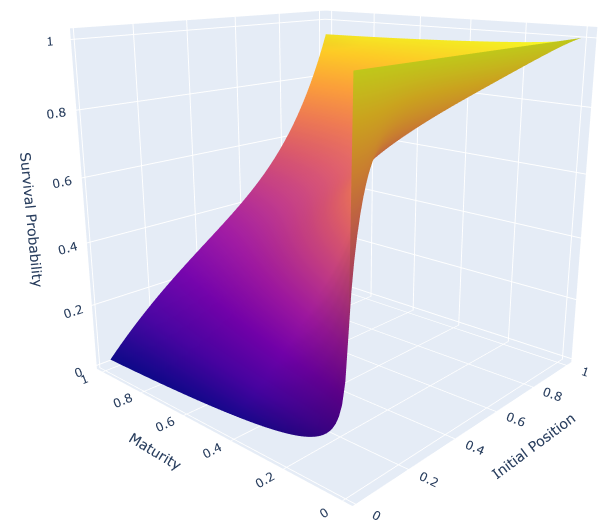
\includegraphics[height= 60mm, width=70mm,scale=0.3]{PD_example_5_3_1.png}
			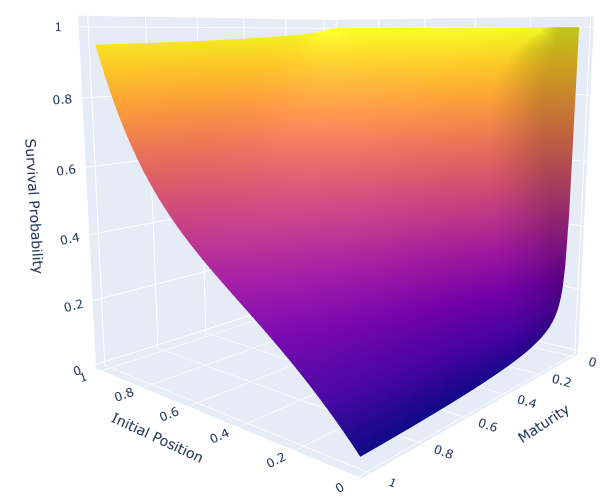
\includegraphics[height=60mm, width=68mm, scale=0.3]{PD_example_5_3_2.png}
		\end{center}
		\caption{Survival probability using the BTCS scheme.}
		\label{fig:btcs_fig_1}
	\end{figure}
\end{example} \hfill $\triangleleft$
\begin{remark}
	In addition to the schemes above, relavant research has focused on implicit handling of the jump term and/or Crank-Nicolson schemes. We omit these methods from the present work, as they are not the main focus, however we refer the interested reader to \cite{d2005robust}, \cite{jwo2020investigation} or \cite{carr2007numerical}. 
\end{remark}

\subsection{Numerical Scheme for the Regime-switching model}
We now turn to the regime-switching model. By considering an implicit scheme we can obtain the BTCS discretized version of $(\ref{int-markov})$. Let $\Phi^q_{p,s}$ represent the survival probabibility at the grid point $t_q=t_0+ q\Delta t$, $x_p=x_0+p\Delta x$, when the underlying Markov process originally in state $r$, i.e. $\Phi^q_{p,s}=\Phi(x_p,t_q,s)$. Considering that the process starts at rating state $R_0=1$, we get:
\begin{eqnarray}
-\lambda \Delta t I^q_{p,1} - \Phi_{p,1}^q = (ra + \frac{1}{2} br \Delta x) \Phi^{q+1}_{p+1,1} + (-\lambda \Delta t - 1 - 2ra + \Delta t q_{12} + \Delta t q_{13}) \Phi_{p,1}^{q+1} +\nonumber\\ (ra-\frac{1}{2}br\Delta x) \Phi_{p-1,1}^{p+1} - \Delta t \big(q_{12} \Phi^{q+1}_{p-1,2} + q_{13} \Phi^{q+1}_{p-1,3}\big).
\end{eqnarray}
Employing the matrix notation as in the original implicit scheme, the regime-switching PIDE can be written as:
\begin{eqnarray} \label{matrix-form}
 \bf{M'}\bf{\Phi}^{q+1} = \bf{\Lambda}' \bf{\Phi}^q+ \bf{b}', 
\end{eqnarray}
where we define the block-form matrices
	\begin{eqnarray} \notag
\bf{\Phi}^{q} =\left[ \begin{array}{c}
\Phi^q_1 \\
\\
\Phi^q_2 \\
\\
\Phi^q_3\\
\end{array}
\right]
b'=\left[\begin{array}{c}
b \\
b \\
0_3 \\
 \end{array}
\right]
M'=\left[  \begin{array}{ccc}
M & -\Delta t q_{12} I_{p \times p}  & -\Delta tq_{13} I_{p\times p } \\
-\Delta t q_{21} I_{p\times p}  & M & -\Delta t q_{23} I_{p\times p}  \\
0_{p\times p} & 0_{ p \times p} &  I_{p\times p} \\
\end{array}
\right]
\Lambda '=\left[  \begin{array}{ccc}
  \Lambda  &0_{p\times p} & 0_{p\times p} \\
 0_{p\times p} &\Lambda& 0_{p\times 3}  \\
0_{p\times p} & 0_{p\times p} &  0_{p\times p} \\
\end{array}
\right],
\end{eqnarray}
where $\Phi_i ^ q = (\Phi_{1,i}^q, \dots \Phi_{1,N}^q)^T$ and $b, M, \Lambda$ are as in (\ref{matrices_1}) and (\ref{matrices_2}). Also note that when $R_t=3$, corresponding to the absorbing default state, the transition probability to any other state and the survival probability is zero.

\subsubsection{Stability and monotonicity}

\begin{example}\label{ex_rs}
Consider an asset process governed by the regime-switching model below: 
 \begin{eqnarray} 
 	dG_t =  
 	\begin{cases} 
 		  0.3(0.7 -x)dt +0.5dB_t + \int_{z\in \mathbb{R}} z N(dt,dz) \text{ if $S_t=$Stage 1,}   \\
 		  0.1(0.4 -x)dt +0.9dB_t + \int_{z\in \mathbb{R}} z N(dt,dz) \text{ if $S_t=$Stage 2,} \\
 	\end{cases}
 \end{eqnarray}
 	where, as in Example \ref{ex}, the Compound Poisson Processes both have normally distributed jumps, with size $Z \sim N(0.0,0.5)$ and rate $\lambda = 1.0$. We have also set $N=1000, T= 100$ for the space and time grids, respectively. Furthermore, the transition matrix of the underlying Markov process given by:
$$Q=\left(  \begin{array}{ccc}
	-0.5 & 0.3  & 0.2 \\
	0.3  & -0.6 & 0.3  \\
	0.0 & 0.0 &  0.0 \\
\end{array}
\right).$$
The graphs in Figure (\ref{graphs_rs}) display the estimated survival probability in each regime (Stage), resulting from solving scheme $(\ref{matrix-form})$. 

\begin{figure}[h]
	\begin{center}
		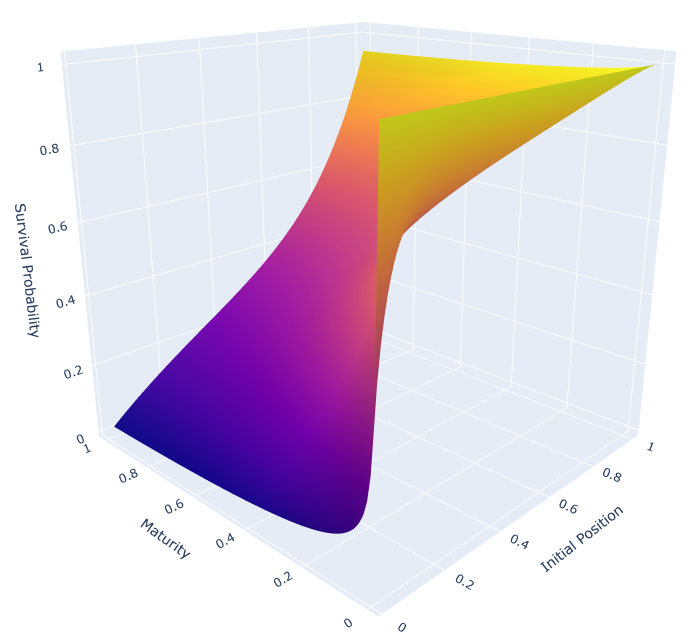
\includegraphics[height=58mm, width=58mm,scale=0.3]{PD_example_5_5_1.png}
		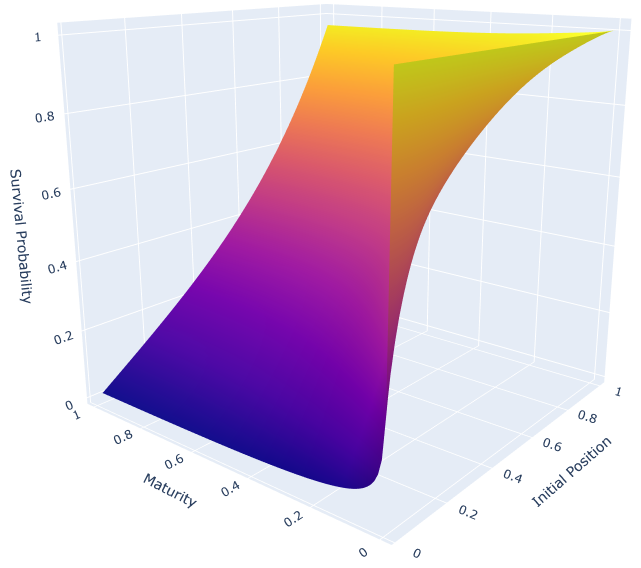
\includegraphics[height=58mm, width=57mm, scale=0.3]{PD_example_5_5_2.png}
		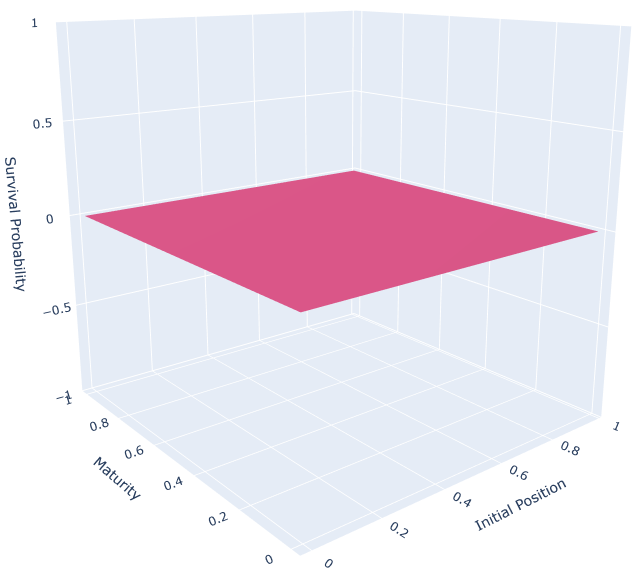
\includegraphics[height=58mm, width=58mm, scale=0.3]{PD_example_5_5_3.png}
		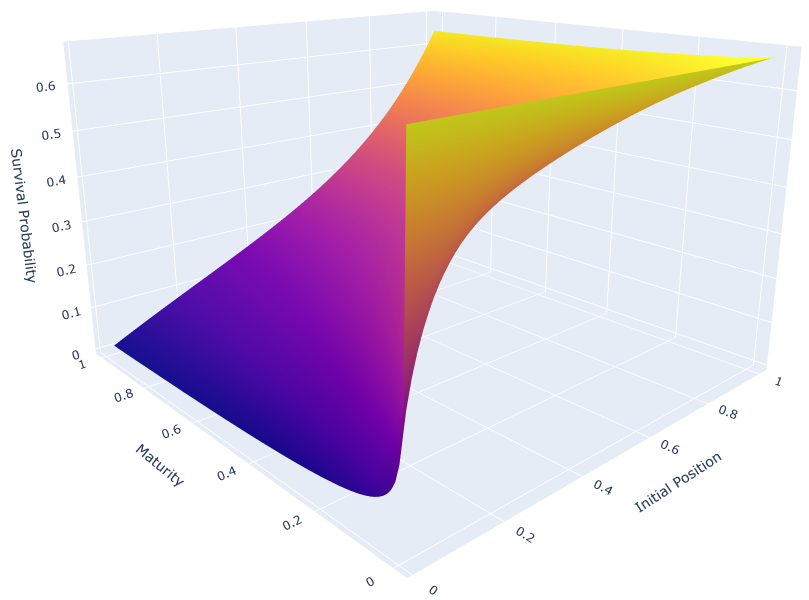
\includegraphics[height=58mm, width=58mm, scale=0.3]{PD_example_5_5_av.png}
	\end{center}
	\caption{Survival probability for Stage 1 (right), Stage 2 (middle), Stage 3 (right), using the BTCS scheme.}
	\label{graphs_rs}
\end{figure}
\end{example}\hfill $\triangleleft$




\begin{comment}
\subsection{Numerical Scheme for the Stochastic volatility model}
In the case of the PIDE driven by stochastic volatility, we must consider appropriate grids for time, space, as well as the volatility process. To do this, we consider a grid of length $D$ for $y$, with $y_j = y_0 + j \Delta y$. Hence, we will estimate the survival probability at distinct points on the three-dimensional grid, for which we will use the notation $ \Phi^q_{p,j}=\Phi(x_p,t_q,y_j)$. Substituting into ($\ref{pide-sv}$) and rearranging, we obtain the following BTCS scheme for the stochastic volatility:
\begin{eqnarray} \label{scheme-sv}
-\lambda \Delta t I^q_{p,j} - \Phi_{p,j}^q =\Big (\frac{1}{2} r_1 \Delta x k (\theta -x) + \frac{1}{2} r_1 y\Big) \Phi^{q+1}_{p+1,j} + (-\lambda \Delta t - 1 - r_1y-r_2\xi^2y) \Phi_{p,j}^{q+1} +\nonumber\\ \Big(-\frac{1}{2}r_1\Delta x k(\theta -x) + \frac{1}{2}r_1y\Big) \Phi_{p-1,j}^{p+1} +\Big(\frac{1}{2}r_2\Delta y \theta_1(\omega-y)+ \frac{1}{2}y\xi^2\Big)\Phi^{q+1}_{p,j+1} \nonumber\\ +\Big(-\frac{1}{2}r_2\Delta y \theta_1(\omega-y)+\frac{1}{2}r_2y\xi^2\Big) \Phi^{q+1}_{p,j-1} 
\end{eqnarray}
where $r_1 = \frac{\Delta t} {\Delta x^2}$ and $r_2 = \frac{\Delta t} {\Delta y^2}$. The solution of the scheme will result in estimations of the survival probability at each state of the underlying stochastic volatility process. Therefore, the resulting vector $\Phi$ will be $ND$ dimensional, where recall $N$ is the length of the $x$-grid. In matrix block form we can write (\ref{scheme-sv}) as in (\ref{matrix-form}) with $\Phi^q, b'  \in \mathbb{R}^{ND}$ and $M,N \in \mathbb{R}^{ND\times ND}$:
	\begin{eqnarray} \notag
\bf{\Phi}^{q} =\left[ \begin{array}{c}
\Phi^q_{1,1} \\
\Phi^q_{2,1} \\
\vdots\\
\Phi^q_{m,1}\\
\vdots\\
\Phi^q_{1,n}\\
\Phi^q_{2,n}\\
\vdots\\
\Phi^q_{m,n}\\
\end{array}
\right],
\,\,\,\,
b'=\left[\begin{array}{c}
b \\
b \\
\vdots \\
b \\
\end{array}
\right],
\,\,\,\,
M=\left[  \begin{array}{ccccccc}
M_1 & 0 & 0  & 0& 0 &\cdots &  0 \\
S_l  & M_2 & S_u & 0 & 0 &\cdots & 0  \\
0 & S_l & M_3 & S_u & 0 & \cdots & 0 \\
\vdots &  \vdots & \vdots & \vdots  & \vdots & \vdots & \vdots \\
0 & 0 & 0  &0& 0 &\cdots &  M_m \\

\end{array}
\right], \,\,\,\,
\Lambda=\left[  \begin{array}{ccccc}
N  & 0 & \cdots &0 & 0\\
0 &N & \cdots  & 0  &0 \\
\vdots &  \vdots & \vdots & \vdots  & \vdots  \\
0 & 0 &  0 & 0& N\\
\end{array}
\right],
\end{eqnarray}
where $M_i, S_l, S_u \in \mathbb{R}^{N \times N}$ are given by:
\begin{eqnarray} \notag
M_i=\left(  \begin{array}{ccccccc}
1 & 0 & 0  & 0& 0 &\cdots &  0 \\
 C & B & A & 0 & 0 &\cdots & 0  \\
0 & C& B & A & 0&\cdots & 0 \\
\vdots &  \vdots & \vdots & \vdots  & \vdots & \vdots & \vdots \\
0 & 0 & 0  &0& 0 &\cdots &  1\\
\end{array}
\right), \,\,\,
S_l=\left(  \begin{array}{ccccccc}
0 & 0 & 0  & 0& 0 &\cdots &  0 \\
0 & \alpha & 0 & 0 & 0 &\cdots & 0  \\
 0& 0 & \alpha& 0 & 0 & \cdots & 0 \\
\vdots &  \vdots & \vdots & \vdots  & \vdots & \vdots & \vdots \\
0 & 0 & 0  &0& 0 &\cdots &  0\\
\end{array}
\right), \,\,\,
S_u=\left(  \begin{array}{ccccccc}
0 & 0 & 0  & 0& 0 &\cdots &  0 \\
0 & \beta & 0 & 0 & 0 &\cdots & 0  \\
0& 0 &  \beta & 0 & 0 & \cdots & 0 \\
\vdots &  \vdots & \vdots & \vdots  & \vdots & \vdots & \vdots \\
0 & 0 & 0  &0& 0 &\cdots &  0\\
\end{array}
\right),
\end{eqnarray}
with the entries given by the coefficients of the BTCS scheme, i.e. $C = -\frac{1}{2}r_1\Delta x k(\theta -x) + \frac{1}{2}r_1y $, $B= -\lambda \Delta t - 1 - r_1y-r_2\xi^2y$, $C=\frac{1}{2} \Delta x k (\theta -x) + \frac{1}{2} r_1 y$ and $\alpha = \frac{1}{2}r_2\Delta y \theta_1(\omega-y)+\frac{1}{2}r_2y\xi^2$, $\beta =\frac{1}{2}r_2\Delta y \theta_1(\omega-y)+ \frac{1}{2}y\xi^2$. 


\begin{example}\label{ex_sv}
Consider an asset process following the stochastic-volatility model: 
\begin{eqnarray}  
	\begin{cases} 
		dG_t = 0.7(1.0 -x)dt +Y_tdB_t + \int_{z\in \mathbb{R}} z N(dt,dz), \\
		dY_t = 0.5(0.5- Y_t)dt  + \sqrt{Y_t}dW_t, \,\,\,\ Y_0=0.1,\\
	\end{cases}
\end{eqnarray}
where the Compound Poisson Process has normally distributed jumps, with size $Z \sim N(0.0,0.5)$ and rate $\lambda = 1.0$. Furthermore, we select $N=400$ and $T=100$ for the space and time grids, respectively, as well as a 50-step grid for the volatility variable $y$, i.e. $D=50$ with $Y_0 = 0.1, Y_{50} = 0.999$. The results are displayed in Figure \ref{graphs_sv}. 

\begin{figure}[h]
	\begin{center}
		%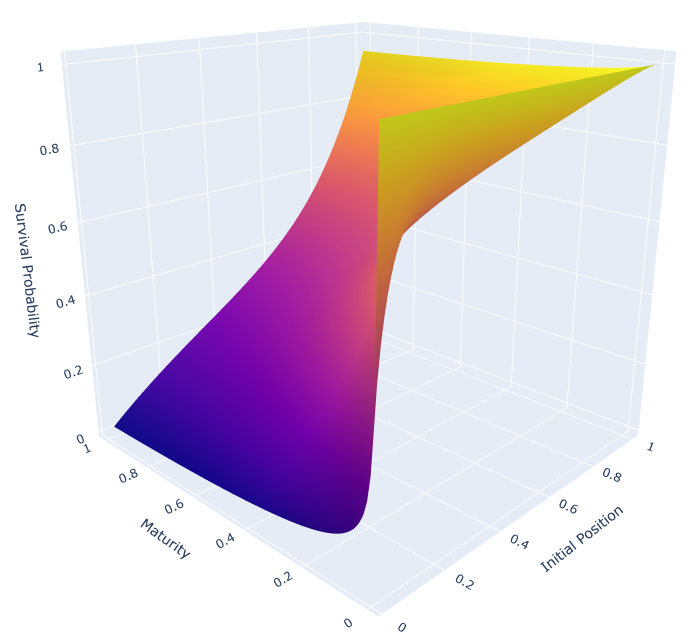
\includegraphics[height= 55mm, width=55mm,scale=0.3]{PD_example_5_5_1.png}
		%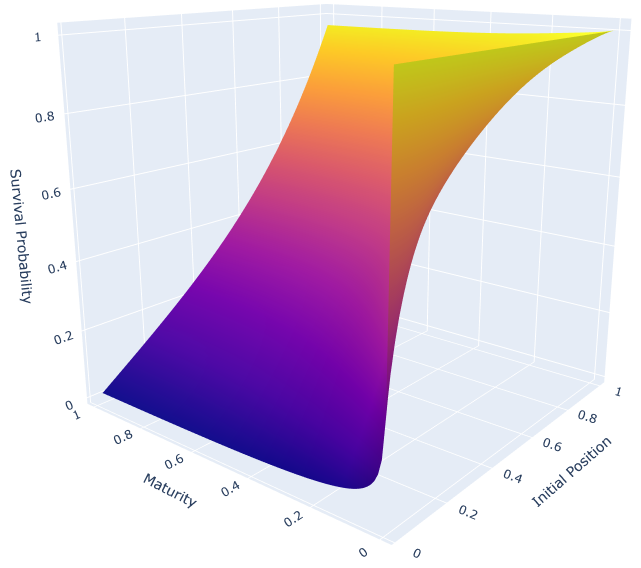
\includegraphics[height=55mm, width=55mm, scale=0.3]{PD_example_5_5_2.png}
		%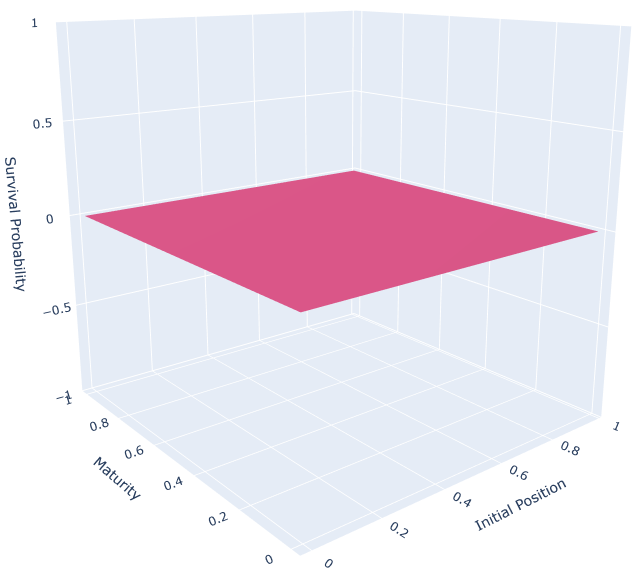
\includegraphics[height=55mm, width=55mm, scale=0.3]{PD_example_5_5_3.png}
	\end{center}
	\caption{Survival probability under the stochastic volatility model using the BTCS scheme.}
	\label{graphs_sv}
\end{figure}

\end{example}\hfill $\triangleleft$
\end{comment} 


\section{Applications to IFRS 9}
The IFRS 9 framework now requires provision calculations to take into consideration multiple risk factors and their evolution. Using the term structure of the PD process, we can estimate provisions for Stage 1 and Stage 2 loans. Provisioning calculations depend on the risk parameters of the loan; the PD process and Loss Given Default (LGD), as well as the amortization schedule, which affects the Exposure at Default (EAD), i.e. the remaining value of the loan which is not repaid in the case of default. Under IFRS 9, financial institutions must account for additional provisions for loan exposures which display a significant increase in credit risk. 
\par These forward-looking lifetime provisions must be calculated per exposure, with some minor differences depending on the type of portfolio (e.g. for corporate loan portfolios many consider contamination effects). In this section, we display how the framework outlined above can be used to calculate the provisions under IFRS 9. The main contribution is the calculation of Lifetime provisions for Stage 2 exposures which, as previously stated, is a novel requirement introduced by the these regulatory standards. We provide specific examples of provision calculations for each case below. 

\subsection{Stage 1 Provisions}
For Stage 1 loans, standard regulations apply and we need only consider losses that can be incurred on the current exposure. This calculation is given by the simple formula:
\begin{eqnarray}\label{stage_1_losses}
 \mathbb{E}[L_t]:=EL_t = EAD_t LGD_t PD_t.
\end{eqnarray}
Using the implicit numerical schemes we can calculate the current PD value as:
$$ PD_t = \Psi(x,t,t+1),$$ where the above represents the survival probability, given the starting point $x$ at time $t$, with maturity $t+1$. Hence, this calculation only account for the probability that the loan defaults in the next period. A simple example for various starting points for the asset process is given below.

\begin{example}
	Consider a Stage 1 loan, with parameters of the asset process as given in Example \ref{ex} and fixed maturity. Then, depending on the initial position of the asset at the time of loan origination, the provisions are calculated in Table \ref{Tab:prov_s1}.
	$$ EL = 100\cdot PD \cdot 75\% $$
\begin{center}
	\begin{tabular}{@{} *{7}{c} @{}}
		\headercell{Initial Position} & $PD_t$ & $LGD$ & Provisions\\
		%\cmidrule(l){2-7}
		\midrule
		$0.0$  & 1.0000 &  0.75 &  75.00\%  \\
		$0.1$  & 0.5219 &  0.75 &  39.14\%  \\
		$0.2$  & 0.2464 &  0.75 & 18.48\%  \\
		$0.3$  & 0.1347 &  0.75 &  10.10\%  \\
		$0.4$  & 0.1007	&  0.75 &  7.55\% \\
		$0.5$  & 0.0924 &  0.75 &  6.93\%  \\
		$0.6$  & 0.0905 &  0.75&   6.79\% \\
		$0.7$  & 0.0891 &  0.75 &  6.68\%  \\
		$0.8$& 0.0845  &  0.75 & 6.34\%   \\
		$0.9$  & 0.0678 &  0.75 &  5.09\%  \\
		$1.0$ & 0.0000  &  0.75 & 0.00\%   \\
	\end{tabular}
\captionof{table}{Provision calculations for Stage 1 loan, given initial position of the asset process.}
\label{Tab:prov_s1}
\end{center}
Hence, if, at the time of calculation, the asset process is estimated to start at $x=0.2$, the provisions are $18.48\%$ of the current exposure.
\noindent
	\hfill $\triangleleft$
\end{example}
As expected, the provisions are a decreasing function of the initial position. A similar table can be produced at any point during the lifetime of the loan, by estimating the corresponding PD values. We also note that, in practice, the LGD could also be a function of the initial position, and/or be correlated to the PD process. Examples using such assumptions are given in e.g. \cite{miu2006basel}, \cite{witzany2011two}. As our focus is the PD process, in this and subsequent examples we will be considering a constant LGD, for simplicity.

\subsection{Stage 2 Provisions}
We now turn to loan provision calculations for Stage 2 loans. Under IFRS 9, if and when loans transition to Stage 2, the lender is obligated to consider all future losses for provisioning purposes. Hence, at any time $t$, and assuming discrete amortization payments, the following formula for the expected losses occuring at some time $i > t$:
\begin{eqnarray}
	\mathbb{E}[L_i] = \mathbb{E} \Big[ \frac{1}{(1+r_i)^{i-t}} LGD_i PD^{PiT}_i EAD_i | \mathcal{F}_t\Big],
\end{eqnarray}
and the correspondining formula for the Lifetime Expected Credit Losses (ECL) at time $t$:
\begin{eqnarray}\label{ECL}
\text{ECL}_t =  \mathbb{E} \Big[\sum_{i=t+1}^{T} \frac{1}{(1+r_i)^{i-t}} LGD_i PD^{PiT}_i EAD_i | \mathcal{F}_t\Big],
\end{eqnarray}
where $r_i$ is the interest rate at time $i$ and $T$ 
the maturity. In the above, $PD^{PiT}_i$ represents the conditional Point in Time PD, which is the probability of default occuring at a given future time period. Specifically, we define:
\begin{eqnarray} \label{pitpd}
	PD^{PiT}_s =  \mathbb{P}\big(\inf_{\substack{s-1 \leq u \leq s}} G_u^x \leq 0, \inf_{\substack{t \leq u \leq s-1}} G_u^x > 0\big),
\end{eqnarray} 
for $s \geq t $. Without loss of generality, we will consider a starting time $t=0$. In order to calculate the $PD^{PiT}$ in terms of the PD proces resulting from the solution of the PIDE, we note that:
$$  \mathbb{P}\big(\inf_{\substack{0 \leq u \leq s}} G_u^x \leq 0) = \mathbb{P}\big(\inf_{\substack{0 \leq u \leq s-1}} G_u^x \leq 0) + \mathbb{P}\big(\inf_{\substack{s-1 \leq u \leq s}} G_u^x \leq 0, \inf_{\substack{0 \leq u \leq s-1}} G_u^x > 0\big),$$ and hence:
$$PD^{PiT}_s  = \Psi(x,s)  -\Psi(x,s-1) = \Phi(x,s-1)  -\Phi(x,s),$$ %where we have written $\Psi, \Phi$ rather than $\tilde{\Psi},\tilde{\Phi}$, for brevity. 
Therefore, (\ref{ECL}) can now be written as:
\begin{eqnarray} \label{ecl2}
\text{ECL} = \sum_{i=1}^{T}\big(\Phi(x,i-1)  -\Phi(x,i)\big)\mathbb{E} \Big[\frac{LGD_i  EAD_i}{(1+r_i)^{i-t}} | \mathcal{F}_t \Big]
\end{eqnarray}
\begin{example}\label{stp}
 Consider a credit exposure with asset process as in Example \ref{ex}. However, we now suppose the exposure has been transferred to Stage 2, with remaining maturity $T = 10$ years. We also consider that the asset process of the borrower is currently estimated at $x=0.2$. To estimate the Stage 2 provisions we require the term structure of the PD process and use ($\ref{ecl2}$) (note that in the table below we consider $r=0$ for simplicity):\\
 
\begin{center}
	\begin{tabular}{@{} *{8}{c} @{}}
		\headercell{Time} &$EAD_t$ & $\Psi(x,t)$ & $PD_t^{PiT}$ & $LGD$ & $EL_t$\\
		%\cmidrule(l){2-7}
		\midrule
		$1.0$  & 100 &  0.2464  &  0.2464 &75\%  &  18.48\%  \\
		$2.0 $  & 90 &  0.4346 &  0.1882  &75\% & 12.70\%  \\
		$3.0$ & 80 &0.5497 &  0.1151 & 75\% & 6.91\% \\
		$4.0$& 70  & 0.6287	  &  0.0790 & 75\% &  4.15\%\\
		$5.0$  & 60 &  0.6869  &  0.0582 &75\%  &  2.62\% \\
		$6.0 $  & 50 &   0.7313&  0.0444  &75\% & 1.67\%  \\
		$7.0$ & 40 &0.7661 &  0.0348 & 75\% &  1.04\%\\
		$8.0$& 30  & 0.7937	  &  0.0276 & 75\% &  0.62\% \\
		$9.0$ & 20 &0.8159&  0.0222 & 75\% & 0.33\% \\
		$10.0$& 10  & 0.8338&  0.0179 & 75\% &  0.13\% \\ \hline 
		ECL & & & & & 48.65 \%
	\end{tabular}
\captionof{table}{Provision calculations for Stage 2 loan, given an asset process with initial position $x=0.2$.}
\end{center}
The exposure and expected losses are in percentages of the remaining loan value to be repaid. As shown, the current Lifetime provisions are given by the sum of the final column: $ECL = 48.65 \%$. \hfill
$\triangleleft$
\end{example}
Naturally, we expect that when an exposure is classified as Stage 2, the parameters of the underlying asset process may differ. In the example above, we purposely consider the same asset process so as to highlight the differences in the final provision estimations. 

\subsection{Provisions under the regime-switching model}
\par As discussed, the new regalutory framework aims to ensure that all financial institutions have accounted for future losses and abrupt changes in credit risk parameters, which can create severe losses and subsequent liquidity and solvereincy issues, both for institutions and their customers. As risk classification is widely considered as a Markov process both in theory and by practitioners, considering transiton probabilities for loans can allow us to forececast the PD processes and estimate worst-case scenario provisions for loan exposures. We note that, in practice, estimating the parameters of the asset prices under each regime may be difficult. However, many financial institutions consider such models and its mathematical framework is well established, see e.g. \cite{chatterjee2015centre} and \cite{bruche2005estimating}. Another approach is to use historical parameters from Stage 1 and Stage 2 loans to estimate the changes that occur when a loan transitions between Stages. For this example, we will be estimating the provisions under the regime-switching model developed above. To this end, we consider an IFRS 9 compliant transition matrix:
$$
P=\left(  \begin{array}{c|ccc}
\text{IFRS 9 Rating} & \text{Stage 1} & \text{Stage 2} & \text{Stage 3}\\
\hline
\text{Stage 1} & p_{11} & p_{12} & p_{12}\\
\text{Stage 2} & p_{12} & p_{22} & p_{13}  \\
\text{Stage 3} & 0 & 0 &1
\end{array}
\right).
$$
For a loan originating in Stage 1, we can now forecast credit losses by taking into account the probability of a SICR (significant increase in credit risk) event. Under the regime-switching model, in the case of a transition to another Stage, we will need to estimate the PD values for the asset process governed by the new parameters. Using the straightforward notation $\Phi^i$ or $PD^i$ to emphasize the Stage (regime) under which the specific PD value is estimated, we can then define the "Stage-weighted provisions", given by:

\begin{eqnarray} \label{weightedprov}
WP_t = p_{11} EAD_t LGD_t PD^1_t + p_{12} \sum_{i=t}^{T}\big(\Phi^2(x,i-1)  -\Phi^2(x,i)\big)\mathbb{E} \Big[\frac{LGD_i  EAD_i}{(1+r_i)^{i-t}} | \mathcal{F}_t \Big]  \nonumber\\ + p_{13}EAD_tLGD_t,
\end{eqnarray}
where the third term occurs in the case of default (i.e. transition to Stege 3), we have that $PD_t=100\%$. This calculation holds for the case where we consider that the transition to Stage 2 occurs one period (e.g. year) after. However, we can also consider the cases where the deterioration occurs at any point $k>t$. For this calculation we require the $k$-step transition matrix of the underlying rating process, which is known to be $P^k$, whose elements will be symbolized as below:
$$
P^k=\left(  \begin{array}{c|ccc}
\text{IFRS 9 Rating} & \text{Stage 1} & \text{Stage 2} & \text{Stage 3}\\
\hline
\text{Stage 1} & p^k_{11} & p^k_{12} & p^k_{12}\\
\text{Stage 2} & p^k_{12} & p^k_{22} & p^k_{13}  \\
\text{Stage 3} & 0 & 0 &1
\end{array}
\right).
$$
with the understanding that $p^k_{ij}$ represents the $k$-th step transition probability. We then have:
\begin{eqnarray} \label{weightedprovk}
\mathbb{E}[WP_k|\mathcal{F}_t] = p^k_{11} EAD_k LGD_k PD^1_k + p^k_{12} \sum_{i=k}^{T}\big(\Phi^2(x,i-1)  -\Phi^2(x,i)\big)\mathbb{E} \Big[\frac{LGD_i  EAD_i}{(1+r_i)^{i-t}} | \mathcal{F}_t \Big] \nonumber \\
+ p^k_{13}EAD_tLGD_t.
\end{eqnarray}
 At any point, with the dynamics of the underlying Markov process, we can obtain the corresponding $WP_t$ values. This calculation takes the future evolution of the loan, as well as the regime into consideration to provide an estimation that encorporates all scenarios.
 For illustrative purposes, we consider the example below.
 \begin{example}
 In this example, we consider a loan exposure driven by the same asset process as in Example \ref{ex_rs}, which is currently in Stage 1. Again, we consider an initial position of $x=0.3$ and maturity $T=10$, for comparison purposes. Furthermore, consider the IFRS 9 compliant loan transition matrix given by:
 \begin{eqnarray}\label{transmatrix}
 P=\left(  \begin{array}{c|ccc}
 \text{IFRS 9 Rating} & \text{Stage 1} & \text{Stage 2}  & \text{Stage 3}\\
 \hline
 \text{Stage 1} & 0.4 & 0.4 & 0.2\\
 \text{Stage 2} & 0.2 & 0.5 & 0.3 \\
  \text{Stage 3} & 0.0& 0.0 & 1.0 \\
 \end{array}
 \right).
  \end{eqnarray}
We will perform the provisioning scenario analysis by forecasting the Stage-weighted provisions, given by ($\ref{weightedprovk}$) for the next four years. We first calculate the $k-$step transition matrices:
  	\begin{eqnarray} \notag
  P^2=\left( \begin{array}{ccc}
  0.24 & 0.36 & 0.40 \\
 0.18 & 0.33 & 0.49 \\
  0.00 & 0.00 & 1.00\\
  \end{array}
  \right),
  \,\,\,\,
 P^3=\left( \begin{array}{ccc}
  0.168 & 0.276 &0.556 \\
  0.138 & 0.237 & 0.625\\
  0.000 & 0.000 & 1.000\\
  \end{array}
  \right),
  \,\,\,\,
  P^4=\left( \begin{array}{ccc}
  0.1224 & 0.2052 & 0.6724 \\
  0.1026 & 0.1737 & 0.7237 \\
  0.0000 & 0.0000 & 1.0000\\
  \end{array}
  \right).
\end{eqnarray}
At time $t=0$ we consider the forward looking scenarios and can calculate the Stage 1 and Stage 2 provisions. Recall that Stage 1 provisions are given by (\ref{stage_1_losses}). Stage 2 (expected lifetime) provisions are given in column $EL_t$ in Table (\ref{weighted_table}), which also contains the Point-in-Time Stage 1 and Stage 2 PD required to calculate the provisions. 
\begin{center}
	\begin{tabular}{@{} *{8}{c} @{}}
		\headercell{Time} &$EAD_t$ & $\Psi^1(x,t)$ & $\Psi^2(x,t)$ & Stage 1 $PD_t^{PiT}$ &Stage 2 $PD_t^{PiT}$ & $LGD$ & $EL_t$\\
		%\cmidrule(l){2-7}
		\midrule
		$1.0$  & 100 & 0.0196 & 0.1285  &0.0196  &0.1285 &75\%  &  9.64  \\
		$2.0 $  & 90 &   0.0391 &  0.2829 & 0.0195 &0.1544 &75\% & 10.42  \\
		$3.0$ & 80 &  0.0600 &  0.3796 & 0.0209 &0.0967  & 75\% & 5.80 \\
		$4.0$& 70  &  0.0834	  &  0.4391 & 0.0234 &0.0595 & 75\% &  3.12 \\
		$5.0$  & 60 &  0.1092  &  0.4757  & 0.0258&0.0366 &75\%  &  1.65 \\
		$6.0 $  & 50 &   0.1365&  0.4983 & 0.0273&0.0226 &75\% & 0.85  \\
		$7.0$ & 40 &  0.1645 &  0.5123 & 0.0280 &0.0140 & 75\% & 0.42 \\
		$8.0$& 30  &  0.1924 &  0.5209& 0.0279& 0.0086& 75\% &  0.19 \\
		$9.0$ & 20 & 0.2197  &0.5262  &0.0273 &0.0053 & 75\% & 0.08 \\
		$10.0$& 10  & 0.2462 &  0.5295& 0.0265 &0.0033 & 75\% &  0.02 \\
	\end{tabular}
	\captionof{table}{Stage 1 and 2 PDs and Expected Lifetime provisions}
	\label{weighted_table}
\end{center}

Using the Stage 1 PD values we can calculate the Stage 1 provisions at each subsequent time period. We also have the evolution of the Expected Lifetime provisions. The final column below contains the Stage-weighted provisions, calculated by (\ref{weightedprovk}). 
 
 \begin{center}
 	\begin{tabular}{@{} *{8}{c} @{}}
 		\headercell{Time}  &  Stage 1 Provisions & $EL_t$ & $WP_t$\\
 		%\cmidrule(l){2-7}
 		\midrule
 		$1.0$  &  1.47  & 32.19  & 28.46  \\
 		$2.0 $  &  1.32 &22.55 & 35.44   \\
 		$3.0$ &  1.25 &12.13 & 36.92 \\
 		$4.0$& 1.22 &6.33 & 36.76 \\
 	\end{tabular}
 \captionof{table}{Stage-weighted provision calculations}
 \end{center}
 \noindent

 \hfill $\triangleleft$
\end{example}

\section{Further Applications in credit risk modelling}
\subsection{Pricing of Credit Default Swaps}
Another financial field in which the PD process plays a paramount role in credit derivatives pricing. In particular, we consider the fair price of Credit Default Swap (CDS). A default swap is a contract that protects the holder of an underlying swap from the losses caused by the default to the obligation’s issuer. Therefore, the evolution of the PD process can be used for the pricing, hedging and managing of such options. Extensive work has been done on modeling and pricing CDSs, such as in \cite{cariboni2007pricing} and \cite{houweling2005pricing}. Specifically, it can be shown that the price of the CDS is given by:
\begin{eqnarray}
C D S=(1-R)\left(-\int_{0}^{T} e^{-r s} d\Phi(x,s)\right)-c \int_{0}^{T} e^{-r s} \Phi(x,s) ds,
\end{eqnarray}
and the corresponding par spread:
\begin{eqnarray}
c^*=\frac{(1-R)\Big(-\int_{0}^{T} e^{-r s} d\Phi(x,s) \Big)} {\int_{0}^{T} e^{-r s} \Phi(x,s) ds}, 
\end{eqnarray}
where $R$ is the specific recovery rate and $r$ is the risk-free rate. The above expression can be discetized as follows:
\begin{eqnarray}
c^*=\frac{(1-R) \sum_{i=1}^{n} e^{-rt_i} (\Phi(x,t_{i-1})- \Phi(x,t_i))} {\frac{1}{2} \sum_{i=1}^{n}e^{-rt_i} (\Phi(x,t_{i-1}) + \Phi(x,t_i)) \Delta t_i}, 
\end{eqnarray}
where the Trapezoidal rule has been used for the discretization of the denominator. Estimating the price and par rate of CDS therefore requires the term structure of the underlying risk-free and survival probability processes. We present a simplified example, whereby the interest rate is considered constant, as our main focus is the use of the PD values for pricing purposes. 
\begin{example}
 Consider a CDS with maturity $T=10$ years and recovery rate $R=0.5$. The pricing can be done under any of the PD modeling frameworks considered above.

Under the regime-switching model, for which we consider an initial asset process value of $x= 0.7$ and with parameters given by $(\ref{params_regime_switching})$, we obtain the following PD values by averaging across all three regimes at each point of the discretized time grid, along with the corresponding CDS price: 

\begin{center}
	\begin{tabular}{@{} *{2}{c} @{}}
		\headercell{Time} &$\Phi(0.7,t)$ \\
		%\cmidrule(l){2-7}
		\midrule
		$0$  & 100.0\% \\
		$1 $  & 59.17\%   \\
		$2$  & 52.39\% \\
		$3 $  & 47.01\%   \\
		$4$ & 42.97\%  \\
		$5$  & 39.97\% \\
		$6 $  & 37.72\%   \\
		$7$ & 36.04\%   \\
		$8$ &  34.75\%   \\
		$9$  & 33.77\% \\
		$10$ & 33.02\%   \\
	\end{tabular}
\end{center}
\noindent
The resulting par spread is calculated based on the PDs, resulting in a par spread of $c^* = 0.56$.

\hfill $\triangleleft$
\end{example}

\subsection{Credit Portfolio Optimization}
For many financial institutions, one of the most important tasks is securitization of credit exposures. Ultimately, this can be formulated as an optimization problem. The PD process affects the risk of each exposure and, by extension, the corresponding return as well. To this end, we present a simple example to show how such an optimization problem can be solved under the stochastic volatility PD model. 
\begin{example}
Suppose a securitization agency creates a portfolio consisting of loans (or credit derivatives), each with different underlying asset process. The PD processes will differ depending on the loans' (or derivatives') characteristics. Suppose that, for a portfolio of three loans, the corresponding PD process are given by $PD_i, i=1,2,3$. The agency aims to select the investment allocated to each of the credit exposures. The PD processes can be estimated with the approach developed. 

Specifically, the agency then poses the following portfolio optimization problem:	suppose $w_i, i=1,2,3$ and $r_i, i=1,2,3$ represent the weight of total investment allocated to each institution's set of loans and  their average return, respectively (in principal, the rate of returns might depend on the characteristics of the transition matrices). Consider, furthermore, that the required portfolio rate of return is set to be $R$. For the credit exposure $i$, at time $t$, the loss function is given by $L_i(t) = EAD_i(t)LGD_i(t)PD_i(t)$. The total loss function for the agency is then given by $L(t)= \sum_{1}^{3} w_iL_i(t)$. In order to rebalance the portfolio at each period, the securitization agency is then interested in solving a portfolio optimization problem (we present a very simple such problem, which can be solved analytically to illustrate the use of the method). The optimization we consider is the following: \\
\begin{eqnarray*}
	\text{minimize } \mathbb{E}[U(L(t))],  \text{ subject to }\\
	w_1 r_1 + w_2 r_2 + w_3 r_3 = R, \\
	w_1 +w_2 +w_3=1,
\end{eqnarray*} 
for an appropriate loss function $U$. While the following analysis can be extended to any convex loss function, for the sake of simplicity, we illustrate the calculation selecting the quadratic loss function $U(L)=bL^2-L$ (in the sense of a negative utility function). To standardize the optimization problem, we consider that $EAD_i$ is given as a percentage of the original loan value and for simplicity we consider $LGD_i(t) = 1$ for $i=1,2,3$ and all $t$. At any point in time $t$, the expected loss utility is then:
$$ \sum_{i=1}^{3} U(w_iEAD_i)PD_i,$$ where we have omitted the dependance on time for brevity. The agency must optimize the portfolio by solving: 
\begin{eqnarray*}
	\text{minimize } f(w_1,w_2,w_3):= \sum_{i=1}^{3} b(w_iEAD_i)^2-w_iEAD_i, \text{ subject to} \\
	w_1 r_1 + w_2 r_2 + w_3 r_3 = R, \\
	w_1 +w_2 +w_3=1,
\end{eqnarray*} 
This simple quadratic optimization problem can now be solved either analytically or numerically. One can easily obtain the expression for one of the weights, e.g. we find that $w_3^*$ is given by:

$$w_3^* =\frac{PD_1(2bEAD_1^2\delta\epsilon - \epsilon)+PD_2(\gamma-2baEAD_2^2\beta\gamma)-PD_3}{2(bPD_1EAD_1^2\epsilon^2+bPD_2EAD_2^2\gamma^2+bPD_3EAD_3^2)}, $$

where $\beta=\frac{R-r_1}{r_2-r_1}, \gamma=\frac{r_3-r_1}{r_2-r_1}, \delta = \frac{r_2-R}{r_2-r_1}$ and $\epsilon=\frac{r_3-r_2}{r_2-r_1}$. A straightforward substitution using the two conditions will result in the corresponding values $w_1^*$ and $w_2^*$.
We consider the above setting with average returns from each institution's instruments $r=(r_1,r_2,r_3)^T$ and current exposures $EAD=(EAD_1,EAD_2,EAD_3)^T$ given by:
\begin{eqnarray}\notag
r=\left( \begin{array}{c}
0.1 \\
0.3 \\
0.1 \\
\end{array}
\right),
\,\,\,\,
EAD=\left(  \begin{array}{c}
0.9  \\
0.8 \\
0.7 \\
\end{array}
\right).
\end{eqnarray}
In order to obtain the vector containing the PD values, we consider the parameters for each of the three asset classes given in the table below:

\begin{eqnarray}
		dG^1_t=0.3(0.7 - G^1_t)dt + 0.5 dB_t +  \int_{z\in \mathbb{R}} z N(dt,dz), \,\,\ x_0 = 0.6\\
		dG^2_t=0.8(0.5 - G^2_t)dt + 1.0 dB_t +  \int_{z\in \mathbb{R}} z N(dt,dz), \,\,\ x_0 = 0.5\\
		dG^3_t=0.5(0.3 - G^3_t)dt + 0.5 dB_t +  \int_{z\in \mathbb{R}} z N(dt,dz),\,\,\ x_0 = 0.4,
\end{eqnarray}
with $J = 4, \lambda =1$ and jump distributions $Z \sim N(0.0,0.5)$ for all three of the asset processes.
Solving PIDE $(\ref{pide2})$, we obtain the PD values:
$$PD=\left( \begin{array}{c}
0.0905\\
0.1808	\\
0.1027 \\
\end{array}
\right).$$
Fixing the expected total return to be $R=0.25$, the resulting optimal weights $w^*=(w_1^*,w_2^*,w_3^*)^T$ are:

$$w^*=\left( \begin{array}{c}
0.083\\
0.335\\
0.582 \\
\end{array}
\right).$$
%\hfill$\triangleleft$
\end{example}  \hfill $\triangleleft$\\
\par For extensive work on portfolio optimization problems with defaultable assets, we refer the interested reader to e.g. \cite{asanga2014portfolio}. Furthermore, empirical studies of the applicability of standard ruin probabilities in practice can be found in \cite{braun2015solvency}. In the example above, we focus on a case where an agency must assess and optimize a portfolio of loan exposures with varying characteristics. Such cases could be loans originating in different sectors; e.g. in \cite{pasricha2020portfolio}, the authors consider a portfolio of risky bonds originating from the Industry and Service sector.


\section{Conclusion}
In this paper we have foocused on a generalized approach of estimating PD values, considering both the cases of variable starting times and maturities. We show that under certain conditions imposed on the asset process, these two cases can be dealt with by solving a PIDE resulting from the infinitesimal generator of the PD process. We have shown that the numerical solution to the PIDE can be best approximated using an implicit scheme, which also allows us to easily consider any type of jump distribution corresponding to the discontinuity of the asset process. Such methods have important advantages over standard simulation-based approaches, such as Monte Carlo methods, as they do not explicitly depend on the simulated paths.
\par Overall, the proposed framework covers many of the difficulties financial institutions face due to the new regulatory requirements for provision calculations, as well as continuous credit risk monitoring for SICR events. We hypothesize that such an approach would be preferrable for practicioners, as well, given that lengthy simulations are not required to approximate accurate solutions. Furthermore, using the developed approach we can easily obtain point in time and lifetime PDs, each of which are used extensively in credit risk management. Specifically, the framework for this PD estimation is based on the needs created by the IFRS 9 regulations, under which forecasting credit losses accurately and efficiently is of paramount importance. We show how the PD estimations can be used to calculate Stage 2 provisions, as well as more advanced, scenario-based provisions, for which a regime-switching model can be used. Of course, as discussed, this approach is beneficial to further applications such as securitization and pricing. 
\par Specifically for the case of provisions, we note that this approach most likely is best fit for corporate and small business loans, where the estimation of asset processes has been documented in well-established work. Of course, it is possible that with new develops in payment services and Open-Banking solutions (in accordance to the Payment Services Directive 2), such methods could be applied to individual consumers, given sufficient historical data. An example of recent work done in this direction is \cite{tobback2019retail}. Moreover, the LGD parameter is also of great importance for provision calculations; in this work we considered a constant LGD, however, in practice, LGD values require separate model development, often related to current macroeconomic variables, as shown in \cite{bellotti2012loss}. 


\bibliographystyle{plain}
\bibliography{bibliography}

\section{Appendix}
\subsection{Important results for It\^o-L\'evy processes}
\begin{theorem}
	Let $X_t \in \mathbb{R}$ be an It\^o- L\'evy process and consider a function $f(t,x)$, with $f \in C^{2}(\mathbb{R}^2)$. Then, the dynamics of the process $f(t,X_t)$ are given by the following version of the It\^o formula:
	\begin{align*}
	& df(t,X_t) = \frac{\partial f}{\partial t}(t,X_t)dt + \frac{\partial f}{\partial x} (t,X_t) \big(a(t) dt  +  \sigma(t) dB_t \big) + \frac{1}{2} \frac{\partial^2 f}{\partial x^2} (t,X_t) \sigma^2(t) dt \\
	& + \int_{\mathbb{R}} f\big(t,X_{t-}+ H(t,z)\big) - f(t,X_{t-}) N(dt, dz)
	\end{align*}
	\end {theorem}
	
	The above generalization of the It\^o formula for jump processes will allow us to consider the evolution of the PD process, as previously described. However, a necessary condition for the application of the result above is the the differentiability of $f(t,x)$ - specifically $f$ is considered to be twice differentiable in $x$ and once in $t$. This requirement is often not satisfied, creating the need for a version of the formula in the weak sense. This is addressed by the combination of the two following results by \cite{krylov2008controlled} and \cite{okhrati2015ito}, respectively:
	
	\begin{theorem} \label{jump1}  %check
		Consider the stochastic process $$dX_t=a(t,x) dt + \sigma(t,x) d B_{t}$$ and a region $Q$, where $B_t$ is a standard Brownian motion, with function $f$ such that function $f \in W^{1,2}(Q)$. Moreover, let $\tau$ be some Markov time such that $\tau < \tau_Q$, where $t_Q$ is the exit time of the process from the region $Q$.   Then, if there exists some constant $K$ such that $|\sigma(t)|+|a(t)| \leq K$, for some fixed time $s$ we have that:
		\begin{equation}
		\begin{split}
		\MoveEqLeft
		e^{-\varphi_{\tau}} f(s+\tau, X_\tau)-e^{-\varphi_{t}} f(s+t, X_t) = \int_{t}^{\tau} e^{-\varphi_{u}}\frac{\partial f}{\partial u}(s+u, X_u) du\\
		&+\int_{t}^{\tau} e^{-\varphi_u} \frac{\partial f}{\partial x}(s+u, X_u) \sigma(u,X_u) dB(t)
		+\frac{1}{2}\int_{t}^{\tau} e^{-\varphi_{u}} \frac{\partial^2 f(s+u, X_u)}{\partial x^2} \sigma^2(u,X_u) du,
		\end{split}
		\end{equation}
		almost surely.
	\end{theorem}
	
	\begin{theorem} \label{jump2}
		Consider the stochastic process with representation
		$$
		X_t=\gamma t+\int_{0}^{t} \int_{\mathbb{R}} z N(d u, d z),$$
		where $\gamma \in \mathbb{R}$. 
		Assume $f:[0, \infty) \times U \rightarrow \mathbb{R}$ is a continuous function on $[0, \infty) \times U$ such that $f \in L_{loc}^{1}([0, \infty) \times U)$,
		$\operatorname{supp}(f) \subset[0, \infty) \times U$, where $U$ is an open set of $\mathbb{R}$
		with locally bounded weak first order derivatives $\partial^{\alpha}f$, defined by:
		$$ \int_{[0,\infty] \times U} (\partial^{\alpha}f(x))\phi(x)dx = (-1)^{|a|} \int_{[0,\infty] \times U} f(x)(\partial^{\alpha}\phi(x))dx,$$ for all $\phi \in C^{\infty}_c([0,\infty] \times U)$. Then:
		\begin{eqnarray}
		f(t, X_t)=f(0, X_0)+\int_{0}^{t} \frac{\partial f}{\partial s}(u, X_u) d u+\gamma \int_{0}^{t} \frac{\partial f}{\partial x}(u, X_u) du+\nonumber \\ 
		\quad+\int_{0}^{t} \int_{\mathbb{R}}f(u, X_{u-}+z)-f(u, X_{u-}) N(d u, d z),
		\end{eqnarray}
		where all derivatives are understood in the weak sense.
	\end{theorem}


\begin{comment}

\subsection{Numerical scheme for an asset process driven by a subordinator}
In practice, it is often appropriate to consider only negative jumps in the asses process, possibly due to the effect of abrubt changes due to various macroeconomic factors. In such cases, we can consider a subordinator process for the L\'evy jump, with the asset process then described by: 
\begin{eqnarray}\label{gousub}
dG_t^x=k(\theta - G_t)dt + \sigma dW_t -  \int_{z\in \mathbb{R}} z N(dt,dz),
\end{eqnarray}
where the density function $f(z)$ is defined on $\mathbb{R}_+$. The corresponding PIDE is then given by: 
\begin{eqnarray} \label{pide3}
\frac{\partial \Phi}{\partial t}=\frac{1}{2} \sigma^{2} \frac{\partial^{2} \Phi}{\partial x^{2}}+k(\theta-x) \frac{\partial \Phi}{\partial x}  - \lambda \Phi(x,t)+\lambda \int_{0}^{x}\Phi(x-z,u)f(z)dz. 
\end{eqnarray}

For the solution of the PIDE, we can consider a forward time centered space discretization scheme (FTCS), resulting in the explicit finite difference equation below:
\begin{eqnarray} \label{FTDS}
\frac{\Phi_p^{q+1}-\Phi_{p}^{q}}{\Delta t} =\frac{1}{2}\sigma^2 \frac{\Phi_{p+1}^{q}-2  \Phi_{p}^{q}+\Phi_{p-1}^{q}}{(\Delta x)^{2}}+k(\theta-x) \frac{\Phi_{p+1}^{q}-\Phi_{p-1}^{q}}{2 \Delta x}-\lambda\Phi_{p}^{q}+\lambda I^q_p, 
\end{eqnarray}
Then, 
$$I^q_p = \sum_{i=0}^{N} \bar{\Phi}_{p-i}^{q} \bar{f}_{i} \Delta z,$$ with 
upon rearranging (\ref{FTDS}), we obtain the numerical scheme given by:
\begin{eqnarray}
\Phi_{p}^{q+1} = \Phi^q_{p+1}\Big( ra + \frac{1}{2}br \Delta x \Big) + \Phi_p^q(1-2ra - \lambda \Delta t) + \Phi_{p-1}^q \Big( ra - \frac{1}{2}br \Delta x  \Big) + \lambda \Delta t I_p^q.
\end{eqnarray}
Finally, we will need to assess the stability of the scheme. To do this we will consider the Von Neumann stability of the scheme. We conclude that the scheme is conditionally stable,  according to the Proposition below, based on the corresponding result from \cite{abdollahi2019stability}. 
\begin{proposition}
	The FTCS scheme (\ref{FTDS}) is Von Neumann stable  for 
	$$ r:= \frac{\Delta t} {\Delta x^2} \leq \frac{1}{\sigma^2}.$$
\end{proposition}

\begin{proof}
	The proof lies on \cite{abdollahi2019stability} for the PDE:
	\begin{eqnarray} \label{pde}
	\begin{aligned} u_{t}(x, t)=a(x, t) u_{x x}(x, t)+b(x, t) u_{x}(x, t)+c(x, t) u(x, t), && x \in(0,1), \\ && 0\leq t \leq  T, \\ u(x, 0)=\varphi(x), && x \in[0,1] \\ u(0, t)=f(t), && 0 \leq t \leq T\\ u(1, t)=g(t), && 0 \leq t \leq T, \end{aligned}
	\end{eqnarray}
	where $a(x,t) > 0$ and $c(x,t)  \leq 0$. This is proven to be stable for $r \leq \frac{1}{2a(x,t)}$, by the principle of frozen coefficients. In the case of the PD process satisfying $(\ref{pide3})$, since $\int_{0}^{x}\Phi(x-z,u)f(z)dz \leq \Phi(x,t)$, we have that:
	$$ \lambda \int_{0}^{x}\Phi(x-z,u)f(z)dz - \lambda \Phi(x,t) = \mu(x,t)\Phi(x,t),$$
	for some function $\mu(x,t) < 0.$ Substituting into (\ref{pide3}), we obtain the PDE (\ref{pde}), with $$a(x,t):= \frac{1}{2} \sigma^2 >0, \,\,\, b(x,t) := k(\theta - x), \,\,\, c(x,t):= \mu(x,t) < 0$$ and initial conditions $$\phi(x) = \mathbbm{1}_{x>0}, \,\,\, f(t)=0, \,\,\,  g(t) = 1.$$
	In then follows that stability is achieved for $$r \leq \frac{1}{\sigma^2}.$$
\end{proof}


For this case, we consider an exponential distribution with the intensity $\lambda$ for the jump distribution. The parameter values were selected as shown in the table below: 
\begin{center} \label{params}
\begin{tabular}{|l|l|}
\hline
\bf{Parameter} & \bf{Value} \\ \hline
$k$ & 0.1  \\ \hline
$\theta$ & 0.5  \\ \hline
$\sigma$ & 1  \\ \hline
$\lambda$ & 0.2  \\ \hline
$\text{define CPP rate}$ & ****** \\ \hline
\end{tabular}\\
\end{center}
where $\lambda$ is the jump rate of the compound Poisson process. We solve the FTCS (\ref{FTDS}) scheme for a grid with $x_0 =0, x_N =1,\Delta x = 0.02$ and $t_0=0, t_N = 10, \Delta t = \frac{10}{60,000}$, thus ensuring that the stability condiition is satisfied. We obtain the following results: \\
\begin{center}
\begin{tabular}{@{} *{8}{c} @{}}
\headercell{Initial Position} & \multicolumn{6}{c@{}}{Maturity}\\
\cmidrule(l){2-8}
& $0$ & $1$ & $2 $ & $3$ & $\cdots$ & $9$ & $10$   \\ 
\midrule
$0.0$  & 0.0000 &  0.0000 &  0.0000  &  0.0000 & $\cdots$& 0.0000& 0.0000 \\
$0.2$  & 1.0000 &  0.1939 & 0.1914 & 0.1913 &$\cdots$ &  0.1913  & 0.1913 \\
$0.4$  & 1.0000 &  0.3872 & 0.3832 & 0.3831 & $\cdots$ & 0.3831 &0.3831 \\
$0.6$ & 1.0000 & 0.5834&  0.5793 &0.5793&  $\cdots$ & 0.5793 & 0.5793\\
$0.8$& 1.0000  &  0.7862 &  0.7836  & 0.7836& $\cdots$ &  0.7836 & 0.7836 \\
$1.0$ & 1.0000 &  1.0000& 1.0000 & 1.0000  & $\cdots$&  1.0000& 1.0000 \\
\end{tabular}
\end{center}
\noindent
\begin{figure}
\begin{center}
\includegraphics[height= 60mm, width=70mm,scale=0.3]{PD_1.png}
\includegraphics[width=60mm,scale=0.3]{PD_2.png}
\end{center}
\caption{Solution to the FTCS scheme for the survival probability}
\end{figure}
\end{comment}

\end{document}